\documentclass[11pt]{article}

% ARR/*ACL review format: anonymous, line-numbered, page-numbered review PDF.
\usepackage[review]{acl}

\usepackage{times}
\usepackage{latexsym}
\usepackage[T1]{fontenc}
\usepackage[utf8]{inputenc}
\usepackage{microtype}
\usepackage{graphicx}
\usepackage{amsmath}
\usepackage{amsfonts}
\usepackage{booktabs}
\usepackage{multirow}
\usepackage{nicefrac}
\newcommand{\keywords}[1]{\par\noindent\textbf{Keywords:} {\def\and{; }#1}}

\title{Dual-Granularity Gaussian Contrastive Learning \\for Table Union Search}
\author{Anonymous Submission}

\begin{document}
\maketitle

\begin{abstract}
The task of table union search aims to retrieve tables that are unionable with a given query table from large tabular repositories such as data lakes. Despite recent advances, existing methods still face two fundamental limitations: 
(1) the implicit modeling of semantic specificity, where deterministic point embeddings encode only semantic centers while ignoring semantic coverage; and (2) the self-referential bias in contrastive learning, which treats only augmented views as positives and suppresses potentially compatible tables.
To address these issues, we propose DGGC, a Dual-Granularity Gaussian Contrastive Learning framework for table union search. DGGC represents both tables and columns as Gaussian embeddings, explicitly modeling semantic centers and specificity distributions via mean and variance parameters. We further design a unified objective that integrates Gaussian modeling with contrastive learning under a table–column alignment constraint, ensuring consistency between global and local semantics. In addition, a filter–shuffle sample generator constructs diverse inter-table positive pairs, alleviating the closed-world assumption of standard contrastive learning. Extensive experiments on three real-world table corpora demonstrate that DGGC consistently outperforms state-of-the-art baselines while maintaining efficiency.

\keywords{Table union search \and Gaussian embeddings \and Contrastive learning \and Sample generator \and Semantic specificity}
\end{abstract}

\section{Introduction}
\label{intro}
With the rapid growing number of open datasets, data lake becomes a prevalent storage architecture across governments \cite{deng2024lakebench}, data scientists \cite{zhang2020finding}, businesses \cite{halevy2016goods} and enterprises\cite{khatiwada2022integrating}. Web tables constitute a substantial portion of data lakes due to their rich knowledge and semi-structured format \cite{deng2024lakebench}. In the Semantic Web community, table interpretation, tabular entity linking, semantic description induction, and dataset discovery have been extensively studied for exploiting tabular and dataset-level semantics~\cite{bhagavatula2015tabel,efthymiou2017matching,cutrona2020tough,vu2021graph,benjelloun2020google}. Among these tasks, table union search aims to retrieve tables that are unionable with a given query table, serving as a cornerstone for data integration and dataset enrichment \cite{nargesian2018table,zhang2020finding,leventidis2024large}. 

However, tables in data lakes are highly heterogeneous and large-scale, posing challenges to both effectiveness and efficiency. Early approaches design heuristic scoring functions to measure unionability but struggle to capture implicit semantics and structural heterogeneity \cite{nargesian2018table}. Recent representation learning methods leverage pre-trained language models to encode table semantics, with Starmie \cite{fan2022semantics} adopting contrastive learning and a filter–verification framework to compute unionability scores.
\begin{figure}[t]
    \centering
    
    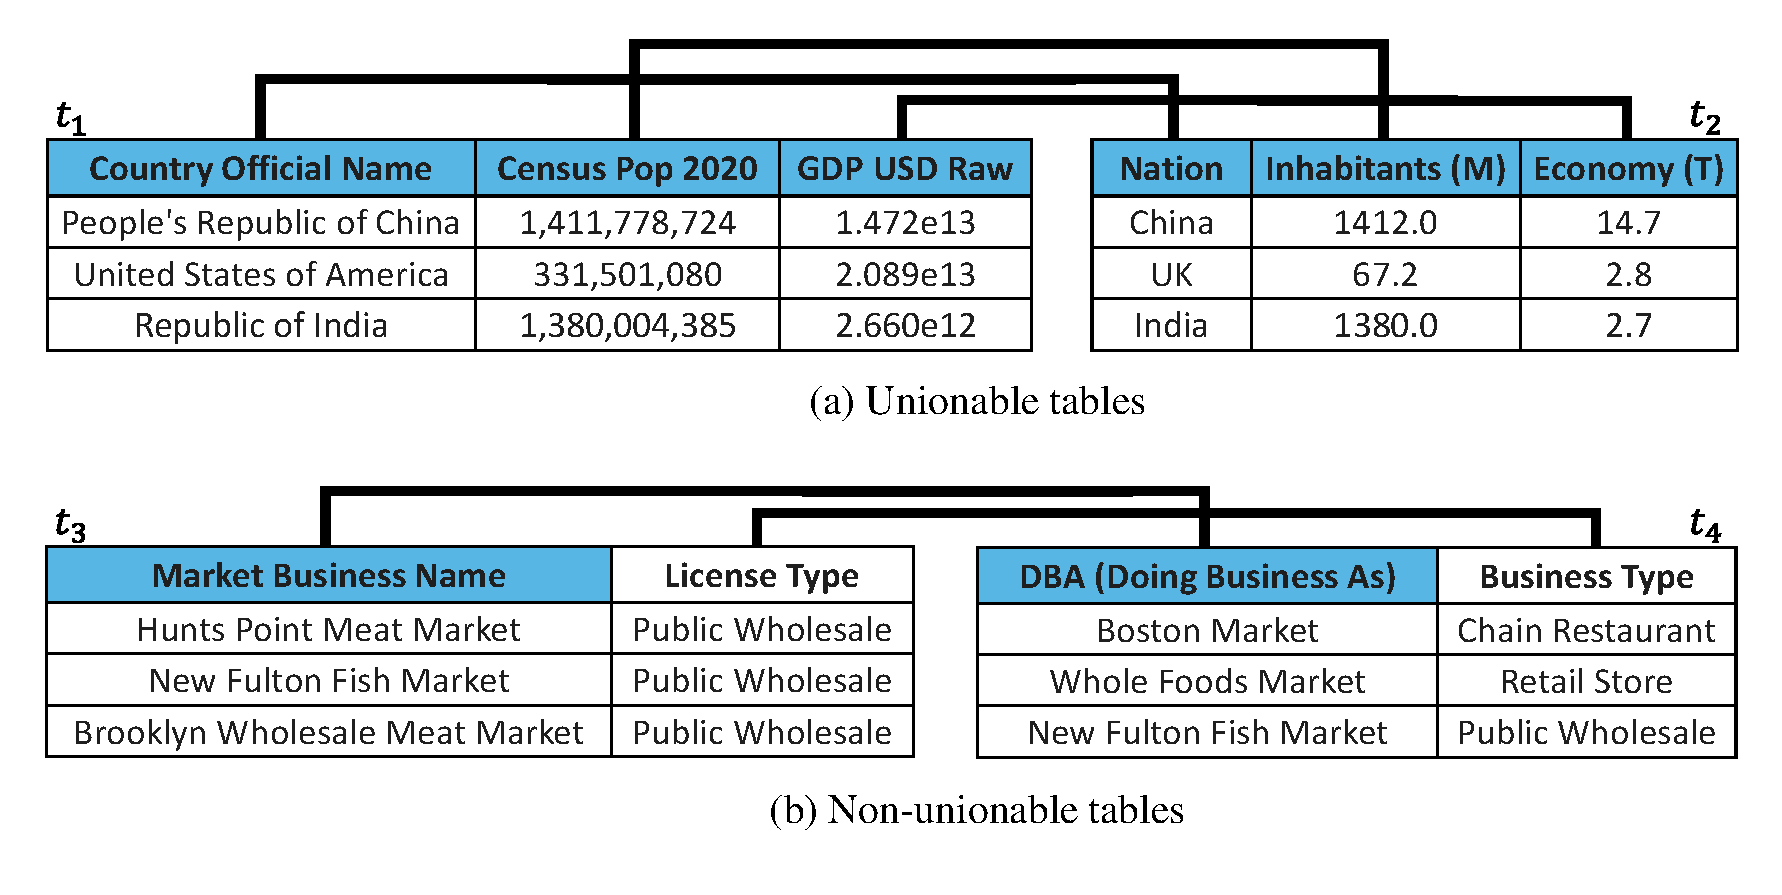
\includegraphics[width=\columnwidth]{figure/intro_example.pdf}
    
    \caption{An example of table union search. The black lines represent the matched columns.}
    
    \label{intro_example}
\end{figure}

Contrastive learning methods provide a self-supervised approach that resolves the lack of a large number of labels for training in table union search, thereby enhancing generalization \cite{fan2022semantics}. However, contrastive learning poses two challenges for table union search: (1) \textit{Implicit representation of semantic specificity.} Most approaches use deterministic point embeddings to encode tables or columns, modeling only semantic centers while ignoring semantic coverage. As illustrated in Figure \ref{intro_example}(b), columns {``Market Business Name''} in $t_3$ and {``DBA (Doing Business As)''} in $t_4$ may refer to the same entity type yet differ in specificity (wholesale markets vs. general markets). When represented as point vectors, such concepts may lie close in embedding space, leading to overestimated unionability. Without explicitly modeling semantic coverage, the boundary between general and specific concepts becomes blurred, resulting in unreliable retrieval decisions; (2) \textit{Self-referential bias in contrastive learning.} Standard contrastive frameworks assume that for an anchor table $t_i$, only its augmented view $t_i'$ is a positive sample, while all other tables are treated as negatives. This closed-world assumption introduces self-referential bias in heterogeneous data lakes \cite{boutaleb2025something}, where semantically compatible tables may coexist without explicit labels. Consequently, unionable tables (e.g., $t_1$ and $t_2$ in Figure \ref{intro_example}(a)) may be penalized as negatives, causing the model to overemphasize self-content and misclassify semantically related but lexically distinct tables.

To address the challenges identified earlier, this paper introduces the \underline{D}ual-\underline{G}ranularity \underline{G}aussian \underline{C}ontrastive Learning (DGGC) framework for table union search. DGGC models both tables and columns as Gaussian embeddings, where mean vectors capture semantic centers and variance vectors quantify semantic specificity. To ensure consistency between global table semantics and local column semantics, DGGC incorporates a table–column alignment objective within a unified Gaussian contrastive learning framework. 
Moreover, we design a filter–shuffle sample generator that constructs diverse inter-table positive pairs by filtering irrelevant tables and shuffling rows within unionable pairs. By extending positive supervision beyond self-augmentation, this strategy mitigates self-referential bias. Extensive experiments on three real-world corpora demonstrate that DGGC consistently improves union search effectiveness while maintaining efficiency.

The main contribution of this paper are summarized as follows:

\noindent $\bullet$\textit{Dual-Granularity Gaussian Contrastive Learning.} We introduce a Gaussian-based contrastive framework that explicitly models semantic specificity distributions at both table and column levels.

\noindent $\bullet$\textit{Filter-Shuffle Sample Generator.} We propose a positive sample generation strategy that constructs inter-table positives to alleviate the self-augmentation limitation in contrastive learning.

\noindent $\bullet$\textit{Experiment Results.} Experiments on three table corpora demonstrate consistent improvements over state-of-the-art methods, supported by ablation studies and case analyses. The reproducibility package is described in the Supplemental Material Statement and code are released in \small{https://anonymous.4open.science/r/DGGC-anonymous-artifact-7A99}. 


The remainder of the paper is organized as follows. Section~\ref{rel_work} reviews related work, Section~\ref{method} presents the proposed method, Section~\ref{exp} reports experimental results, and Section~\ref{cld} concludes the paper.


\section{Related Work}
\label{rel_work}

\subsection{\textbf{Table Union Search}}
Table Union Search (TUS), also known as entity complement~\cite{das2012finding} or row extension~\cite{yakout2012infogather}, aims to discover tables in data lakes that can be vertically extended with a query table~\cite{nargesian2018table}. Existing approaches can be broadly categorized into overlap-based, semantic-based, and distribution-based methods. 

\noindent\textbf{Overlap-based Approaches.}
Early work focuses on value overlap. Research~\cite{nargesian2018table} proposes set-unionability using a hypergeometric test to assess domain similarity. PGTUS~\cite{xie2024pgtus} accelerates such matching via proximity graphs, and Juneau~\cite{zhang2019finding} incorporates multi-view signals including row similarity and header distance. However, overlap-based methods struggle with semantically similar but lexically distinct columns.

\noindent\textbf{Semantic-based Approaches.}
To overcome exact matching limitations, recent studies leverage representation learning. Methods such as Table2Vec~\cite{zhang2019table2vec} and contextual encoders~\cite{pilaluisa2024contextual} map columns into embedding spaces for semantic matching. SANTOS~\cite{khatiwada2023santos} emphasizes relationship semantics across columns, while LifTus~\cite{qiu2025liftus} models multi-aspect features for unseen data lakes. 
Starmie~\cite{fan2023starmie} introduces contrastive learning into TUS by generating positive views through column dropping and row sampling. While effective, such self-augmentation strategies may treat other unionable tables as negatives, leading to self-referential bias. Moreover, most semantic approaches encode tables and columns as deterministic vectors, which compress complex domains into single points and may overlook distributional specificity.

\noindent\textbf{Distribution-based Approaches.}
To capture distributional characteristics, probabilistic and geometric methods have been explored. NL-Unionability~\cite{nargesian2018table} models columns as language distributions, and COTER~\cite{yao2023coter} employs Wasserstein distance for refined alignment. Inspired by this perspective, DGGC represents tables and columns as Gaussian distributions, using mean vectors for semantic centers and variance vectors to model semantic specificity.

\iffalse
\subsection{Table Search}
Beyond union search, table search includes whole table search and table join search. Structure-aware models such as StruBERT~\cite{trabelsi2022strubert}, MTR~\cite{shraga2020web}, and MGNETS~\cite{chen2021mgnets} encode structural dependencies via attention, convolution, or graph networks. Recent generative approaches leverage differentiable indexing~\cite{guo2025birdie} or large language models~\cite{cui2024tablecopilot} for natural language-driven discovery. 
For join search, methods such as Juneau~\cite{zhang2019finding}, correlated top-$k$ matching~\cite{pradhan2023searching}, and AugPath~\cite{gong2025let} explore semantic and multi-hop augmentation paths. These studies highlight the increasing importance of semantic representations in data lake retrieval.

\subsection{Semantic Table and Dataset Search}
Beyond table union search, the Semantic Web community has studied semantic access to tables and datasets from several complementary perspectives. Existing studies link table cells to entities using tabular context~\cite{bhagavatula2015tabel,efthymiou2017matching,cutrona2020tough}, infer table semantics from graph and knowledge base signals~\cite{vu2021graph,qiu2023dependency}, exploit background knowledge for schema matching~\cite{portisch2021background}, and retrieve datasets using metadata or dense ranking models~\cite{benjelloun2020google,chen2023dense}. These works are complementary to this paper, which studies semantic compatibility between query and candidate tables for table union search.
\fi
\subsection{Semantic Table and Dataset Search}

Beyond table union search, the Semantic Web community has studied semantic access to tables and datasets from several complementary perspectives. Existing studies link table cells to entities using tabular context~\cite{bhagavatula2015tabel,efthymiou2017matching,cutrona2020tough}, infer table semantics from graph and knowledge base signals~\cite{vu2021graph,qiu2023dependency}, exploit background knowledge for schema matching~\cite{portisch2021background}, and retrieve datasets using metadata or dense ranking models~\cite{benjelloun2020google,chen2023dense}. Beyond semantic access, table search also includes whole-table search and table join search. Structure-aware models such as StruBERT~\cite{trabelsi2022strubert}, MTR~\cite{shraga2020web}, and MGNETS~\cite{chen2021mgnets} encode structural dependencies via attention, convolution, or graph networks. Recent generative approaches further leverage differentiable indexing~\cite{guo2025birdie} or large language models~\cite{cui2024tablecopilot} for natural language-driven table discovery. For join search, methods such as Juneau~\cite{zhang2019finding}, correlated top-$k$ matching~\cite{pradhan2023searching}, and AugPath~\cite{gong2025let} explore semantic and multi-hop augmentation paths. These studies highlight the increasing importance of structural and semantic representations in data lake retrieval. They are complementary to this paper, which focuses on semantic compatibility between query and candidate tables for table union search.

\subsection{Contrastive Learning over Tables}
Contrastive learning has become a dominant paradigm for table representation learning. Starmie~\cite{fan2023starmie} pioneers its application to table union search by constructing self-augmented positive views. Sudowoodo~\cite{zhang2023sudowoodo} aligns schema and instance representations through self-supervision, and LifTus~\cite{qiu2025liftus} captures fine-grained relationships via hierarchical cross-attention.

However, standard contrastive losses adopt a closed-world assumption in which all non-anchor samples are treated as negatives, potentially repelling valid unionable candidates in dense retrieval settings~\cite{qu2021rocketqa}. Furthermore, contrastive frameworks typically rely on deterministic embeddings that encode only semantic centers. In contrast, DGGC integrates contrastive learning with Gaussian modeling to jointly capture semantic centers and specificity distributions, while constructing inter-table positive pairs to mitigate self-referential bias.
\section{Methodology}
\label{method}
In this section, we define the task and present our proposed Dual-Granularity Gaussian Contrastive Learning (DGGC) model, where the overview of DGGC is illustrated in Figure \ref{fig:over}. We first define the table union search task in Section \ref{sub_pre}. Then we describe the dual-granularity encoder, which explicits tables' and columns' semantic specificity distributions, including a mean embedding and a variance embedding (Section \ref{sub_sec_dul}). Additionally, we design the training loss of Gaussian contrastive learning model (Section \ref{sub_sec_gau}). In Section \ref{sub_sg}, we introduce a filter-shuffle sample generator to expand the positive samples to address the self-referential bias in contrastive learning. The overall training process is presented in Section \ref{sub_sec_over}. Finally, we provide the unionability score between columns and tables for the online search process (Section \ref{sub_sec_onl}).

\subsection{Task Definition}
\label{sub_pre}
\begin{figure*}[t]
    \centering
    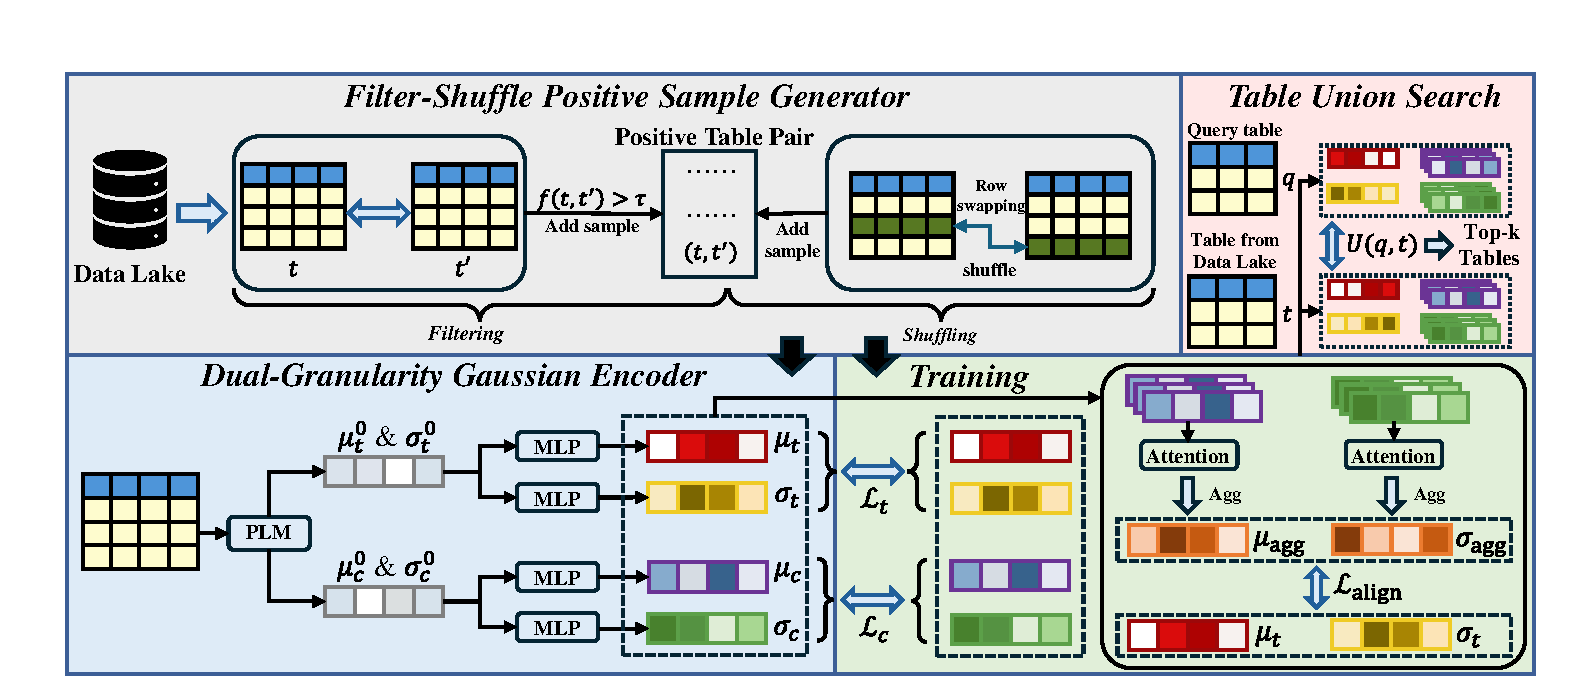
\includegraphics[width=\textwidth]{figure/overview.pdf}
   \caption{
\textbf{The framework of DGGC.} DGGC encodes tables and columns into mean and variance embeddings, uses a filter-shuffle mechanism to generate cross-table positives, and optimizes Gaussian-specific losses for online unionability ranking.
}
    \label{fig:over}
\end{figure*}
Following SANTOS~\cite{khatiwada2023santos}, we adopt a relationship-based semantic definition of unionability. A table is a set of columns $\{c_1,\dots,c_n\}$, each possibly from a distinct domain. Given a query table $q$ and candidate table $t$, $t$ is unionable with $q$ if columns in $q$ can be one-to-one matched to a subset of columns in $t$ while preserving semantic types and inter-column relationships. Accordingly, $U(q,t)$ denotes the semantic unionability degree of $t$ with respect to $q$.
Given a query table $q$ and a table corpus ${T}$, table union search aims to return a top-$k$ list of tables $\{t_1,\dots,t_k\}$ from ${T}$, such that $\forall t\in\{t_1,\dots,t_k\}$ and $\forall t'\in {T}\backslash \{t_1,\dots,t_k\}$, $U(q,t)\geq U(q,t')$.
\subsection{Dual-Granularity Gaussian Encoder}
\label{sub_sec_dul}
Although table union search is typically determined by column similarity, relying solely on column-level representations may ignore global table semantics that provide contextual constraints. To capture both local attribute semantics and global contextual information, we design a dual-granularity Gaussian encoder that models tables and columns simultaneously. To further model semantic specificity beyond deterministic embeddings, we represent each table or column embedding \(x\) as a diagonal Gaussian distribution:
\begin{equation}
\label{eq_gaussian_embedding}
    \mathcal{N}_x
    =
    \mathcal{N}
    \left(
    \mathbf{\mu}_x,
    \mathbf{\Sigma}_x
    \right),
    \qquad
    \mathbf{\Sigma}_x
    =
    \mathrm{diag}(\mathbf{\sigma}_x^2).
\end{equation}
where $\mu_x \in \mathbb{R}^d$ denotes the mean embedding
and $\Sigma_x = \mathrm{diag}(\sigma_x^2)$ is a diagonal covariance matrix. Unlike deterministic embeddings, Gaussian representations allow each table or column to occupy a semantic region in latent space.

We adopt diagonal covariance for scalability, reducing parameter complexity from \(O(d^2)\) to \(O(d)\) and enabling efficient closed-form distance computation.

\noindent\textbf{Initialization.} 
We initialize representations using RoBERTa~\cite{liu2019roberta}, a widely adopted pre-trained language model with strong contextual encoding capability. Pre-trained language models provide rich lexical and contextual priors, which are particularly important for modeling heterogeneous and noisy cell values in data lakes {\cite{yin2020tabert,deng2022turl}}. Each column \(c_i\) is serialized into a sentence \(s_i\) by concatenating its cell values. All column sentences are then organized and the whole table is encoded as $\text{PLM}(\text{[CLS]}\ s_1\ \text{[SEP]} \dots \text{[SEP]}\ s_n \ \text{[SEP]})$, 
where the [CLS] token represents the table-level embedding and each segment corresponds to a column. The PLM output provides initial mean and variance embeddings for both table- and column-level representations, i.e., $\mathbf{\mu}_{t}^0$, $\mathbf{\sigma}_t^0$. For column-level embeddings, the PLM outputs embeddings for each column segment, which are taken as the initial mean $\mathbf{\mu}_{c}^0$ and variance $\mathbf{\sigma}_c^0$ for each column $c$. It is important to note that our approach is applicable to other BERT variants as well. 

\noindent\textbf{Gaussian Layer.} 
After PLM initialization, we use a Gaussian Layer to refine the Gaussian parameters of tables and columns. To avoid ambiguity, we explicitly define four MLP projection functions:
\(\mathrm{MLP}_{t}^{\mu}\), $\mathrm{MLP}_{c}^{\mu}$, $\mathrm{MLP}_{t}^{\sigma}$ and $\mathrm{MLP}_{c}^{\sigma}$. 
The subscript \(t\) or \(c\) denotes the granularity of the input representation, namely table-level or column-level. The superscript \(\mu\) or \(\sigma\) denotes the Gaussian parameter branch, namely the mean branch or the variance branch. Parameters are not shared across granularities or branches to preserve their distinct semantic roles.

For the \(l\)-th Gaussian layer, the mean embeddings are updated as \({\mathbf{\mu}}_{t}^{l+1}=\mathrm{MLP}_{t}^{\mu}(\mathbf{\mu}_{t}^{l})\) and \({\mathbf{\mu}}_{c}^{l+1}=\mathrm{MLP}_{c}^{\mu}(\mathbf{\mu}_{c}^{l})\). Similarly, the variance embeddings are updated as \(\mathbf{\sigma}_{x}^{l+1}=\phi_{\sigma}(\mathrm{MLP}_{x}^{\sigma}(\mathbf{\sigma}_{x}^{l}))\), where \(x \in \{t, c\}\) and \(\phi_{\sigma}\) is a positive activation (e.g., softplus) ensuring valid covariance. In our implementation, \(\phi_{\sigma}\) is instantiated as a softplus function with a small constant \(\epsilon\), i.e., \(\phi_{\sigma}(x)=\mathrm{softplus}(x)+\epsilon\). This positivity constraint guarantees that the diagonal covariance matrix \(\mathbf{\Sigma}_x=\mathrm{diag}(\mathbf{\sigma}_x^2)\) is valid for each table or column Gaussian embedding. Consequently, each table or column is not represented as a single deterministic point, but as a Gaussian distribution with a semantic center \(\mathbf{\mu}_x\) and a specificity-aware covariance parameterized by \(\mathbf{\sigma}_x\).


\subsection{Contrastive Training}
\label{sub_sec_gau}
After obtaining Gaussian embeddings at both table and column granularities, we optimize DGGC with three objectives: table-level contrastive loss, column-level contrastive loss, and a table–column alignment loss. Given a query table \(q\), its unionable tables are treated as positive samples \(\{t_1^+, \dots, t_P^+\}\), while non-unionable tables form the negative set \(\{t_1^-, \dots, t_N^-\}\). The table-level contrastive loss is defined as:
\begin{equation}
\label{eq_cl}
    \mathcal{L}_t=-\log\frac{\sum_{p=1}^P\exp(\mathcal{G}(q,t_p^+))}{\sum_{p=1}^P\exp(\mathcal{G}(q,t_p^+))+\sum_{n=1}^N\exp(\mathcal{G}(q,t_p^-))}    
\end{equation}
For the score function between $q$ and its samples $t$, we adopt the Wasserstein-2 distance as our geometric loss function for Gaussian embedding learning \cite{muzellec2018generalizing}. To flexibly control the relative importance between semantic center alignment and specificity consistency, we introduce a scaling parameter $\lambda$ and define a generalized Wasserstein distance. Given the Gaussian embeddings $\mu_q$, $\sigma_q$ and $\mu_t$, $\sigma_t$ for $q$ and $t$ respectively, we adopt the squared 2-Wasserstein distance between the two Gaussian distributions and convert it into a compatibility score for contrastive learning:
\begin{equation}
\label{eq_gs}
    \mathcal{G}(q,t)=-
    \underbrace{{||\mu_q-\mu_t||_2^2}}_{\text{mean distance}}-\underbrace{\lambda\cdot||\sigma_q-\sigma_t||_2^2}_{\text{variance distance}} 
\end{equation}
where the first term aligns semantic centers and the second enforces consistency of semantic specificity. If the two tables should not be unioned, a penalty of semantic specificity is applied to account for discrepancies in semantic specificity {\cite{vilnis2014word}}. 
The hyperparameter \(\lambda\) controls the relative importance of mean similarity and variance alignment. The introduction of the parameter $\lambda$ serves to balance the importance of mean similarity and variance distance, enabling fine-tuning of the model's sensitivity to semantic discrepancies. The contrastive loss for columns, $\mathcal{L}_c$, is defined analogously to Eq. \eqref{eq_cl} and \eqref{eq_gs}.

To ensure consistency between global table semantics and local column semantics, we aggregate column embeddings within table \(t\). 
For each column \(c \in t\) with Gaussian embedding \((\mu_c, \sigma_c)\), we compute an aggregated table-level representation via attention, where \(\mu_{\text{agg}} = \text{Attn}_{\mu}(\{\mu_{c}\}_{c\in t})\) and \(\sigma_{\text{agg}} = \exp(\text{Attn}_{\sigma}(\{\log\sigma_{c}\}_{c\in t}))\). Here, $\text{Attn}_{\mu}$ and $\text{Attn}_{\sigma}$ are attention functions that compute weighted sums of input embeddings. Using the logarithmic form of variance embeddings stabilizes the variance values and ensures that they are positive, thereby facilitating effective aggregation during the attention computation. Given the Gaussian embedding $\mu_t$ and $\sigma_t$ of table $t$, we define the alignment loss as $\mathcal{L}_{\text{align}}=||\mu_t-\mu_\text{agg}||_2^2+\lambda||\sigma_t-\sigma_\text{agg}||_2^2$. The loss $\mathcal{L}_\text{align}$ reinforces the association of semantic specificity distribution between table and its columns. The total loss is defined as:
\begin{equation}
\label{eq_loss}
\mathcal{L}=\mathcal{L}_t+\alpha\mathcal{L}_c+\beta\mathcal{L}_\text{align}
\end{equation}
where $\alpha$ and $\beta$ are weights to balance different losses.

\iffalse
\subsection{Filter-Shuffle Positive Sample Generator}
\label{sub_sg}
A central difficulty in contrastive learning over heterogeneous tables is \emph{self-referential bias}, where only augmented views of the same table are treated as positives. 
Such a strategy reinforces superficial lexical similarity and fails to expose the model to semantically unionable tables expressed with different surface forms. 
To overcome this limitation, we design a \emph{filter–shuffle} positive sample generator that actively mines high-confidence cross-table positives from the entire data lake.
\fi


\subsection{Filter–Shuffle Positive Sample Generation}
\label{sub_sg}
A central difficulty in contrastive learning over heterogeneous tables is \emph{self-referential bias}, where only augmented views of the same table are treated as positives. 
Such a strategy reinforces superficial lexical similarity and fails to expose the model to semantically unionable tables with different surface forms. 
To address this, we design a \emph{filter–shuffle} positive sample generator that mines high-confidence cross-table positives from the data lake.


\noindent\textbf{Filtering Phase.}
Given two tables $t$ and $t'$, we treat $t$ as the anchor table and evaluate their cross-table compatibility based on column-level alignment quality. 
We first construct a column similarity matrix $A\in\mathbb{R}^{n\times n'}$, where $n$ and $n'$ denote the number of columns in $t$ and $t'$, respectively. 
Each entry $A_{ij}$ quantifies the semantic compatibility between the $i$-th column of $t$ and the $j$-th column of $t'$. We estimate this compatibility from complementary perspectives, capturing lexical similarity of column headers, overlap of cell values, and schema-level structural consistency (e.g., numeric, temporal, or textual). 
All components are normalized into comparable ranges before aggregation.

Based on $A$, we determine the optimal one-to-one column alignment by maximizing the total pairwise compatibility:
\begin{equation}
\label{eq_alignment_strength}
M(t,t') =\frac{1}{n}
\max_{\text{one-to-one column alignments}}
\sum_{i,j} A_{ij}.
\end{equation}
This quantity represents the average alignment strength with respect to the anchor schema, reflecting how well the columns of $t$ can be consistently matched to those of $t'$.

To prevent structurally weak correspondences from being selected, we introduce a minimum compatibility constraint and define
\begin{equation}
\label{eq_filtering_score}
f(t,t') ={M(t,t')}
\cdot\mathbb{I}\!\left[
{M(t,t')} > \gamma
\right],
\end{equation}
where $\gamma$ specifies the minimum average alignment strength required for a pair to be considered structurally coherent. The function $\mathbb{I}[\cdot]$ is an indicator function to return $1$ when its argument is true and $0$ otherwise. 
The indicator term suppresses table pairs whose alignment quality is too low, thereby avoiding matches driven by a small number of coincidentally similar columns. Finally, a table pair is selected as a positive sample if it satisfies 
$f(t,t') > \tau$ and ranks within the top-$K$ candidates for the anchor table.

\iffalse
Since automatically mined positives inevitably vary in reliability, treating all retained pairs uniformly may blur fine-grained semantic distinctions. 
To mitigate this effect, we construct a strength-aware semantic relation map in which each retained table pair is weighted by its filtering score $f(t,t')$. 
Pairs exhibiting stronger and more consistent column-level alignment exert greater influence during training, while weaker pairs contribute proportionally less. 
This adaptive weighting stabilizes contrastive learning under heterogeneous table distributions and reduces the impact of imperfect matches.
\fi

Beyond filtering, \(f(t,t')\) serves as a confidence score for the retained
positive pairs. Because it is computed from the average one-to-one column
alignment strength and is further constrained by \(\gamma\), a higher
\(f(t,t')\) indicates a more reliable cross-table correspondence. We therefore
store each retained pair with its \(f(t,t')\) value in the semantic relation
map and use this score to guide positive sampling during training. In this
way, strongly aligned table pairs are sampled more often, while pairs close to
the filtering boundary have less influence. This prevents automatically mined
positives from being treated uniformly and reduces the effect of noisy
cross-table matches.

\noindent\textbf{Shuffling Phase.}
After obtaining retained positive table pairs from the filtering phase, we
further construct shuffled positive samples to reduce self-referential bias.
For each retained pair \((t,t')\), we reuse the one-to-one column alignment
identified during filtering. Row-wise swapping is performed only on these
aligned columns. Specifically, for a row in \(t\), we randomly sample a row
from \(t'\) and replace the values of the aligned columns in \(t\) with the
corresponding values from the sampled row in \(t'\). Columns that are not
included in the alignment are excluded from the shuffled view to avoid
introducing semantically incoherent attributes.

We repeat this operation for \(r\) rounds, where \(r\) is set to \(30\%\) of
the number of rows in the smaller table. The resulting shuffled table is used
as a positive view of the anchor table. Since the swapping operation is
restricted to columns aligned in the filtering phase, the generated sample
preserves the semantic correspondence between \(t\) and \(t'\) while introducing
lexical and value-level variation. This expands the positive sample space
beyond self-augmentation and exposes the model to semantically related tables
with different surface forms.

\subsection{Overall Learning Process}
\label{sub_sec_over}
DGGC is trained in an end-to-end manner. 
For each mini-batch, tables are first encoded into Gaussian representations at both table and column granularities as described in Section~3.2. 
The filter–shuffle mechanism then identifies reliable cross-table positives and corresponding negatives within the batch. 
Based on these relations, we jointly optimize the table-level contrastive loss, column-level contrastive loss, and table–column alignment loss defined in Section~3.3. 
All model parameters are updated by minimizing the combined objective in Eq. \eqref{eq_loss}. Through this unified training process, DGGC learns specificity-aware representations that remain consistent across granularities while preserving cross-table discriminability.

\subsection{Representations for Table Union Search}
\label{sub_sec_onl}
We now describe the inference procedure for table union search. 
The online scoring function is designed to approximate the semantic unionability principle defined in Section~\ref{sub_pre}, enforcing one-to-one column alignment under consistent semantic type and relational structure. At inference time, unionability is evaluated using the same Wasserstein geometry employed during training, ensuring geometric consistency between optimization and retrieval.


Given two columns $c$ and $c'$ with Gaussian embeddings $(\mu_c,\sigma_c)$ and $(\mu_{c'},\sigma_{c'})$, we use the Wasserstein-based compatibility score $\mathcal{G}(c,c')$ defined in Section~3.3, which jointly captures semantic center alignment and specificity consistency. We operationalize table unionability through a strict alignment principle: a candidate table is considered unionable only if all aligned columns exhibit strong semantic compatibility. 
Formally, the unionability score between a query table $q$ and a candidate table $t$ is defined as
\begin{equation}
\label{eq_union}
    U(q,t)=\exp\!\big(\mathcal{G}(q,t)\big)\cdot\min_{(c',c)\in B}
\exp\!\big(\mathcal{G}(c',c)\big),
\end{equation}
where $\mathcal{G}(q,t)$ is computed analogously from table-level Gaussian embeddings. 
The exponential transformation ensures positivity while preserving the ordering induced by the compatibility measure. 
The minimum operator acts as a bottleneck aggregator, enforcing that weakly aligned columns significantly reduce the overall unionability score. To obtain the column alignment set $B$, we construct a weighted bipartite graph between the columns of $q$ and $t$ using $\exp(\mathcal{G})(c',c)$ as edge weights and compute the maximum-weight bipartite matching via the Hungarian algorithm~\cite{kuhn1955hungarian}. 
The resulting matching {\small\(
B=
\big\{
(c_1',c_1),\dots,(c_i',c_i),\dots,
(c_{{n'}}',c_{{n}})
\big\},
\)}
where $c_i'\in q$ and $c_i\in t$. We implement the bipartite matching using the Hungarian algorithm \cite{kuhn1955hungarian}. 
Finally, candidate tables are ranked according to $U(q,t)$, and the top-$k$ results are returned.

\section{Experiment}
\label{exp}
\subsection{Settings}
\noindent\textbf{Systems.} %这一段主要写你用了什么设备，可以参考
All experiments are conducted on a server with 2 NVIDIA GeForce RTX 3090 GPUs, an AMD EPYC 7513 32-Core Processor, 128GB RAM, Linux, and CUDA 12.2. We implement DGGC in Python using PyTorch and Hugging Face Transformers~\cite{wolf2020transformers}.

\noindent\textbf{Datasets.} We validate the effectiveness of DGGC on three benchmark datasets derived from real-world open data: SANTOS Small \cite{khatiwada2023santos}, TUS Small \cite{nargesian2018table}, and TUS Large \cite{nargesian2018table}. Besides, we employ the SANTOS Large \cite{khatiwada2023santos} and WDC (1M) datasets \cite{lehmberg2016large} exclusively for efficiency evaluation, where we randomly sampled 80 and 300 query tables, respectively. Detailed statistics of these table corpora are presented in Table \ref{tab:datasets}.

\iffalse
We evaluate the effectiveness of our proposed model on three benchmark datasets derived from real-world open data: SANTOS Small, TUS Small, and TUS Large. These datasets are widely utilized in table union search and data integration tasks. Detailed statistics regarding the data lake tables and query tables for each benchmark are presented in the table above.

The SANTOS Small benchmark \textbf{[x]} comprises 550 data lake tables collected from open data repositories in Canada, the UK, the US, and Australia. It includes 50 query tables used to search for unionable candidates. In terms of data scale, the data lake contains a total of 6,322 columns, with tables having an average of 6,921 rows. The query tables are substantial, averaging 21,402 rows per table across 615 columns.

The TUS (Table Union Search) benchmarks \textbf{[x]} are derived from Canadian open data. We utilize two variations: TUS Small and TUS Large. The TUS Small dataset consists of 1,526 data lake tables and 125 query tables. This subset features 14,806 columns in the data lake with an average table size of 3,832 rows. To evaluate scalability and performance on a broader scope, we use the TUS Large benchmark, which scales up to 5,044 data lake tables derived from 32 base tables. It contains a significantly higher dimensionality with 54,950 columns in the data lake and utilizes 100 query tables for evaluation.
\fi


\begin{table}[t]
  \centering
  \caption{Statistics of datasets}
  \label{tab:datasets}
  \resizebox{\columnwidth}{!}{%
  \begin{tabular}{l|ccc|ccc}
    \toprule
    \multirow{2}{*}{\normalsize{Corpus}} & \multicolumn{3}{c}{Data Lake Tables} & \multicolumn{3}{|c}{Query Tables} \\
    %\cline{2-7}
     & \#Tabs & \#Cols & AVG\#Rows & \#Tabs & \#Cols & AVG\#Rows \\
    \midrule
    SANTOS Small & 550 & 6,322 & 6,921 & 50 & 615 & 21,402 \\
    TUS Small & 1,526 & 14,806 & 3,832 & 125 & 1,610 & 4,623 \\
    TUS Large & 5,044 & 54,950 & 1,914 & 100 & 1,792 & 2,108 \\
    \midrule % <--- 在这里添加了线
    SANTOS Large & 11,090 & 123,477 & 7,675 & 80 & 1017& 7675\\
        WDC (1M) & 1M & $\approx$5M & $\approx$15 & 300 & 3680& 8096\\
    \bottomrule
  \end{tabular}%
  }%
\end{table}

\noindent\textbf{Baselines.} %参考starmie中的5.1.4节。
For evaluation on table union search, we compare against the several baselines, including table union search-specific models (D$^3$L \cite{bogatu2020dataset}, SANTOS \cite{khatiwada2023santos}, Starmie \cite{fan2022semantics}, LIFTus \cite{qiu2025liftus}) and PLM-based models (Sherlock \cite{hulsebos2019sherlock}, SATO \cite{zhang2019sato}, TAPAS \cite{herzig2020tapas}, Doduo \cite{jiang2024doduo}). The details about these baselines are presented in Appendix Besides, we also validate the DGGC only with the header input and the values input without headers, i.e., DGGC (only header) and DGGC (only value).

\noindent\textbf{Metrics.}
Consistent with standard evaluation protocols in table union search \cite{khatiwada2023santos,fan2022semantics,qiu2025liftus}, we quantify the effectiveness of top-k result using Mean Average Precision at $k$ (MAP@k) and Recall at $k$ (R@k). All reported scores represent the average across $5$ repeated experimental runs.  

\noindent\textbf{Configuration.} %给出主要参数的取值。最前面还要写一些你训练用的信息，例如说训练样本多大，batch size多大这种。
We employ RoBERTa-base~\cite{liu2019roberta} as the backbone. We use AdamW~\cite{loshchilov2019decoupled} with learning rate \(1e^{-5}\), batch size 64, maximum sequence length 128, and Gaussian embedding dimension 128. For the filter-shuffle generator, the effects of \(\tau\), \(\gamma\), and \(K\) are analyzed in Section~\ref{sec_param_analysis}. Unless otherwise specified, we set \(\lambda=0.5\), \(\alpha=1.0\), and \(\beta=1.0\). For evaluation, we use FAISS~\cite{johnson2019billion} with a Flat Index for exact similarity search.

\subsection{Overall Performance}
\begin{table}[t]
  \centering
  
  \caption{The performance of table union search. The best results are in bold.}
  \label{overall}
  
  \resizebox{\columnwidth}{!}{%
  \begin{tabular}{ll|cc|cc|cc}
    \toprule 
    \multicolumn{2}{c|}{\multirow{2}{*}{Method}}&\multicolumn{2}{c|}{SANTOS-Small}&\multicolumn{2}{c|}{TUS-Small}&\multicolumn{2}{c}{TUS-Large}\\
    &&MAP@k&R@k&MAP@k&R@k&MAP@k&R@k\\
    \midrule
    \multirow{4}{*}{\rotatebox{90}{TUS}}&D$^3$L &.5583&.4517&.6271&.3080&.4847&.1240\\
    & Starmie& .9420& .7700& .9144& .3960& .8670&.2790
\\
 & LIFTus& .9579& .7386& .9623& .3671& .9388&.2702\\
 
    &SANTOS&.9320&.6960&.8780&.3720&.6447&.2983\\
    %&LIFTus&&&.976&.298&.964&.262&.
    \hline
    \multirow{4}{*}{\rotatebox{90}{PLM}}&Doduo&.9039&.6731&.8217&.1033&.8087&.2967\\
    &TAPAS&.3412&.2575&.2061&.1007&.1058&.0513\\
 & Sherlock& .7820& .4930& .9540& .2650& .7440&.1190\\
 & SATO& .8780& .5940& \textbf{.9660}& .2710& .9300&.2230\\
    \hline
    \multirow{3}{*}{\rotatebox{90}{DGGC}}&only header&.9197&.6910&.9288&.3548&.9364&.3241\\
    &only value&.8456&.7089&.9509&.3442&.9375&.3195\\
    &full&\textbf{.9950}&\textbf{.8107}&.9591&\textbf{.3960}&\textbf{.9591}&\textbf{.3610}\\
  \bottomrule
  \end{tabular}%
  }%
\end{table}
To assess the performance of DGGC in capturing table semantics, we conducted a comparative analysis against state-of-the-art baselines across three standard benchmarks. Table ~\ref{overall} presents the MAP@k and R@k performance. Consistent with the settings in prior literature, we set $k=10$ for the SANTOS-Small benchmark and extended $k=60$ for the TUS benchmarks to accommodate the larger search space. %This experimental design facilitates a comprehensive evaluation of the model's robustness across varying scales, ranging from curated small-scale repositories to extensive, noise-intensive data lakes. 

As shown in Table \ref{overall}, DGGC exhibits superior performance, achieving state-of-the-art results on 5 out of 6 evaluated metrics. Specifically, on the SANTOS Small dataset, DGGC reaches a near-optimal MAP@k of 0.9950, outpacing LIFTus (0.9579) and Starmie (0.9420). In TUS-Small, although SATO has a slight edge in MAP@k (0.9660 vs. 0.9591), DGGC demonstrates broader semantic coverage, matching the highest R@k of 0.396 and exceeding SATO's R@k (0.2710) by a significant margin. For TUS-Large, DGGC sets a new benchmark with a MAP@k of 0.9591 and R@k of 0.361, outperforming LIFTus by 2.1\% in MAP@k (0.9591 vs. 0.9388) and surpassing the SANTOS baseline by about 48.7\% (0.9591 vs. 0.6447). Remarkably, DGGC achieves a 61.8\% relative improvement over SATO in R@k (0.3610 vs. 0.2230). These results indicate that the DGGC framework, with its Gaussian embeddings and filter-shuffle sample generator, effectively captures the semantic specificity of tables and columns while mitigating the self-referential bias often encountered in contrastive learning approaches. %removing the variance embeddings (\textit{w/o var}) leads to a catastrophic performance drop on TUS-Large (MAP@k .9591 vs. .3185), demonstrating that explicit uncertainty modeling is paramount for handling the noise in large-scale retrieval. We also observe substantial declines when excluding the Wasserstein penalty (\textit{w/o wass}) or the hard positive mining strategy (\textit{w/o real pos}), confirming their critical roles in aligning semantic manifolds and learning discriminative features. Finally, 
The superior performance of the \textit{full} model over single variants in sample generator (\textit{only header/value}) highlights the necessity of fusing both schema and content information for robust representation. %A detailed analysis of the ablation study is presented in Section \ref{Ablation Study}.

\iffalse
\subsection{Ablation Study}
We perform an ablation study to understand the impact of our key innovations, i.e., the dual-granularity Gaussian embedding, Wasserstein loss, and the filter-shuffle positive sample generator. We compare the full version of DGGC with a version without the filter-shuffle positive sample generator (DGGC w/o FS) and a version without the variance embeddings (DGGC w/o Var). Figure~\ref{fig:ablation_study} shows these comparisons in detail.

As demonstrated in Figure \ref{fig:ablation_study}, DGGC consistently obtains the best results across all benchmarks. On TUS-Large, DGGC w/o Var yields a lower MAP@60 (0.8546) compared to DGGC (0.9090). This decline occurs because the point-based model cannot effectively capture the variance of tables and columns, thereby ignoring the critical influence of semantic specificity.

For the variant without the filter-shuffle sample generator (DGGC w/o FS), we observe a marked performance degradation on smaller datasets. Specifically, on TUS-Small, removing the filter-shuffle mechanism causes the MAP@k to drop drastically from 0.9186 to 0.8251. A similar trend is observed on SANTOS-Small, where DGGC w/o FS (0.9338) falls behind the full DGGC model (0.9954). This suggests that the filter-shuffle sample generator is essential for alleviating the sparsity of positive samples, particularly in data-scarce environments.

%In contrast, DGGC is able to handle those queries and hence, maintain the overall performance. 
%This suggests that the filter-shuffle sample generator helps DGGC alleviate the effect from limited positive samples especially in smaller datasets. \textcolor{red}{more reasons and analysis}

\noindent\textbf{Modeling Semantic Specificity.} The significant performance degradation of the DGGC w/o Var variant on the TUS-Large dataset underscores the inherent limitations of point embeddings when navigating large-scale data lakes. This deficiency stems from the inability of point-based representations to capture semantic scope and asymmetrical unionability relations \cite{vilnis2014word}. In massive table corpora, many candidate tables appear highly proximal in the mean semantic space $\mu$, yet exhibit substantial disparities in their entity coverage or attribute granularity. Conventional point embedding models focus exclusively on the semantic center, leading to semantic over-generalization. In the realm of representation learning, this phenomenon is characterized as a classic semantic compression loss arising from a lack of distributional modeling \cite{muzellec2018generalizing}. In contrast, DGGC explicitly defines semantic boundaries for each table by introducing variance embeddings $\sigma$ and a Wasserstein distance-based penalty. This specificity-aware mechanism enables more precise unionability pruning in complex semantic spaces.

%In contrast, DGGC explicitly defines semantic boundaries for each table by introducing variance embeddings $\sigma$ and a Wasserstein distance-based penalty $\lambda \cdot ||\sigma_q - \sigma_t||_2$. Within this framework, we utilize Gaussian layers to refine and update the initial mean $\mu^0$ and variance $\sigma^0$ provided by the PLM. 
%Specifically, the variance embeddings are mapped via multi-layer perceptrons (MLPs) and a softmax function, a process designed to distill surface-level features into latent uncertainty measures. This transformation converts the initial representations into statistics that characterize the semantic specificity distribution.
%This allows each table and column to be appropriately represented as a multivariate Gaussian distribution. In this mechanism, the mean $\mu$ represents the central semantic tendency, while the refined variance $\sigma$ characterizes the semantic specificity distribution. This specificity-aware mechanism enables more precise unionability pruning in complex semantic spaces, effectively balancing mean similarity and variance distance through the Wasserstein metric.
\noindent\textbf{Mitigating Self-Reference Bias.} The precipitous decline in performance observed for the DGGC w/o FS variant on TUS-Small and SANTOS-Small corroborates the detrimental impact of \textit{self-reference bias} inherent in standard contrastive learning frameworks \cite{robinson2021contrastive}. In the absence of the Filter-Shuffle (FS) generator, the model is susceptible to overfitting on ``literal repetitions'' or simple augmented views \cite{chen2020simple}. By integrating the FS mechanism, the training process is enriched with a multitude of hard positives constructed via row swapping. This augmentation strategy compels the encoder to transcend surface-level token overlaps, focusing instead on capturing deep, invariant structural patterns.
%\textbf{Mitigating Self-Reference Bias. }The precipitous decline in performance observed for the DGGC w/o FS variant on TUS-Small (where MAP plummeted from 0.9186 to 0.8251) and Santos-Small further corroborates the detrimental impact of \textit{self-reference bias} inherent in standard contrastive learning frameworks \cite{robinson2021contrastive}.In the absence of the Filter-Shuffle (FS) generator, the model is susceptible to overfitting on ``literal repetitions'' or simple augmented views \cite{chen2020simple}, thereby failing to capture intrinsic cross-table semantic correspondences. By integrating the FS mechanism, the training process is enriched with a multitude of hard positives constructed via row swapping \cite{robinson2021contrastive}.

%Mechanistically,  while these samples exhibit high lexical diversity derived from distinct table pairs, they maintain structural semantic consistency through the interchange of row values. This augmentation strategy compels the encoder to transcend surface-level token overlaps, focusing instead on capturing deep, invariant structural patterns, a capability that is particularly indispensable for establishing robust feature representations in data-scarce scenarios characteristic of smaller datasets. 

\noindent\textbf{Dual-Granularity Alignment.} The comprehensive superiority of DGGC is further underpinned by the Table-Column Alignment Loss ($\mathcal{L}_{align}$), which enforces a rigorous hierarchical consistency between global and local semantic views \cite{hjelm2018learning}. This dual-granularity constraint acts as a semantic regularizer that prevents the global table embedding from drifting due to irrelevant or noisy columns. In data-scarce environments like TUS-Small and SANTOS-Small, this alignment reinforces feature stability by grounding the high-dimensional table representation strictly in its constituent parts.

%\textbf{Dual-Granularity Alignment.} The comprehensive superiority of DGGC across diverse benchmarks is further underpinned by the Table-Column Alignment Loss ($\mathcal{L}_{align}$), which enforces a rigorous hierarchical consistency between global and local semantic views \cite{hjelm2018learning}. By leveraging an attention mechanism to aggregate column-level features into a cohesive global representation, the model ensures that the macro-level table specificity distribution acts as a faithful, bottom-up aggregation of micro-level column semantics \cite{yang2016hierarchical}. 

%This dual-granularity constraint is particularly pivotal when navigating the high heterogeneity of TUS-Large. It functions as a semantic regularizer that prevents the global table embedding from drifting due to irrelevant or noisy columns, thereby maintaining precise semantic boundaries even amidst extensive schema variations. Conversely, in data-scarce environments like TUS-Small and Santos-Small, this alignment reinforces feature stability by grounding the high-dimensional table representation strictly in its constituent parts. This effectively mitigates the risk of overfitting often observed in decoupled architectures \cite{iida2021tabbie}. Consequently, this synergy not only elevates discriminative power but also endows the model with the robustness required to maintain high retrieval stability across varying data scales.


%To better understand the contribution of the Gaussian constraint and the graph structure, we analyze the performance gain of DGGC relative to the variants. We systematically evaluate how each component compensates for the limitations of the baseline. Furthermore, it shows the significance of both the geometric constraint and the graph module where, the Wasserstein constraint increases DGGC's MAP@k by 6.4\% on TUS-Large over the baseline, and the graph module increases it by 11.3\% on TUS-Small compared to DGGC w/o FS. Similarly, on Santos-Small, the graph structure increases effectiveness by 6.6\% (0.9338 to 0.9954), confirming its critical role. This shows that DGGC w/o Var alone has decent accuracy on large data, but incrementally adding geometric constraints and heterogeneous positive samples improves the accuracy further in a robust trend. Thus, leveraging geometric constraints and structural semantics is benefited by the use of both components.
\fi

\subsection{Ablation Study}
\begin{figure*}[t]
    \centering
    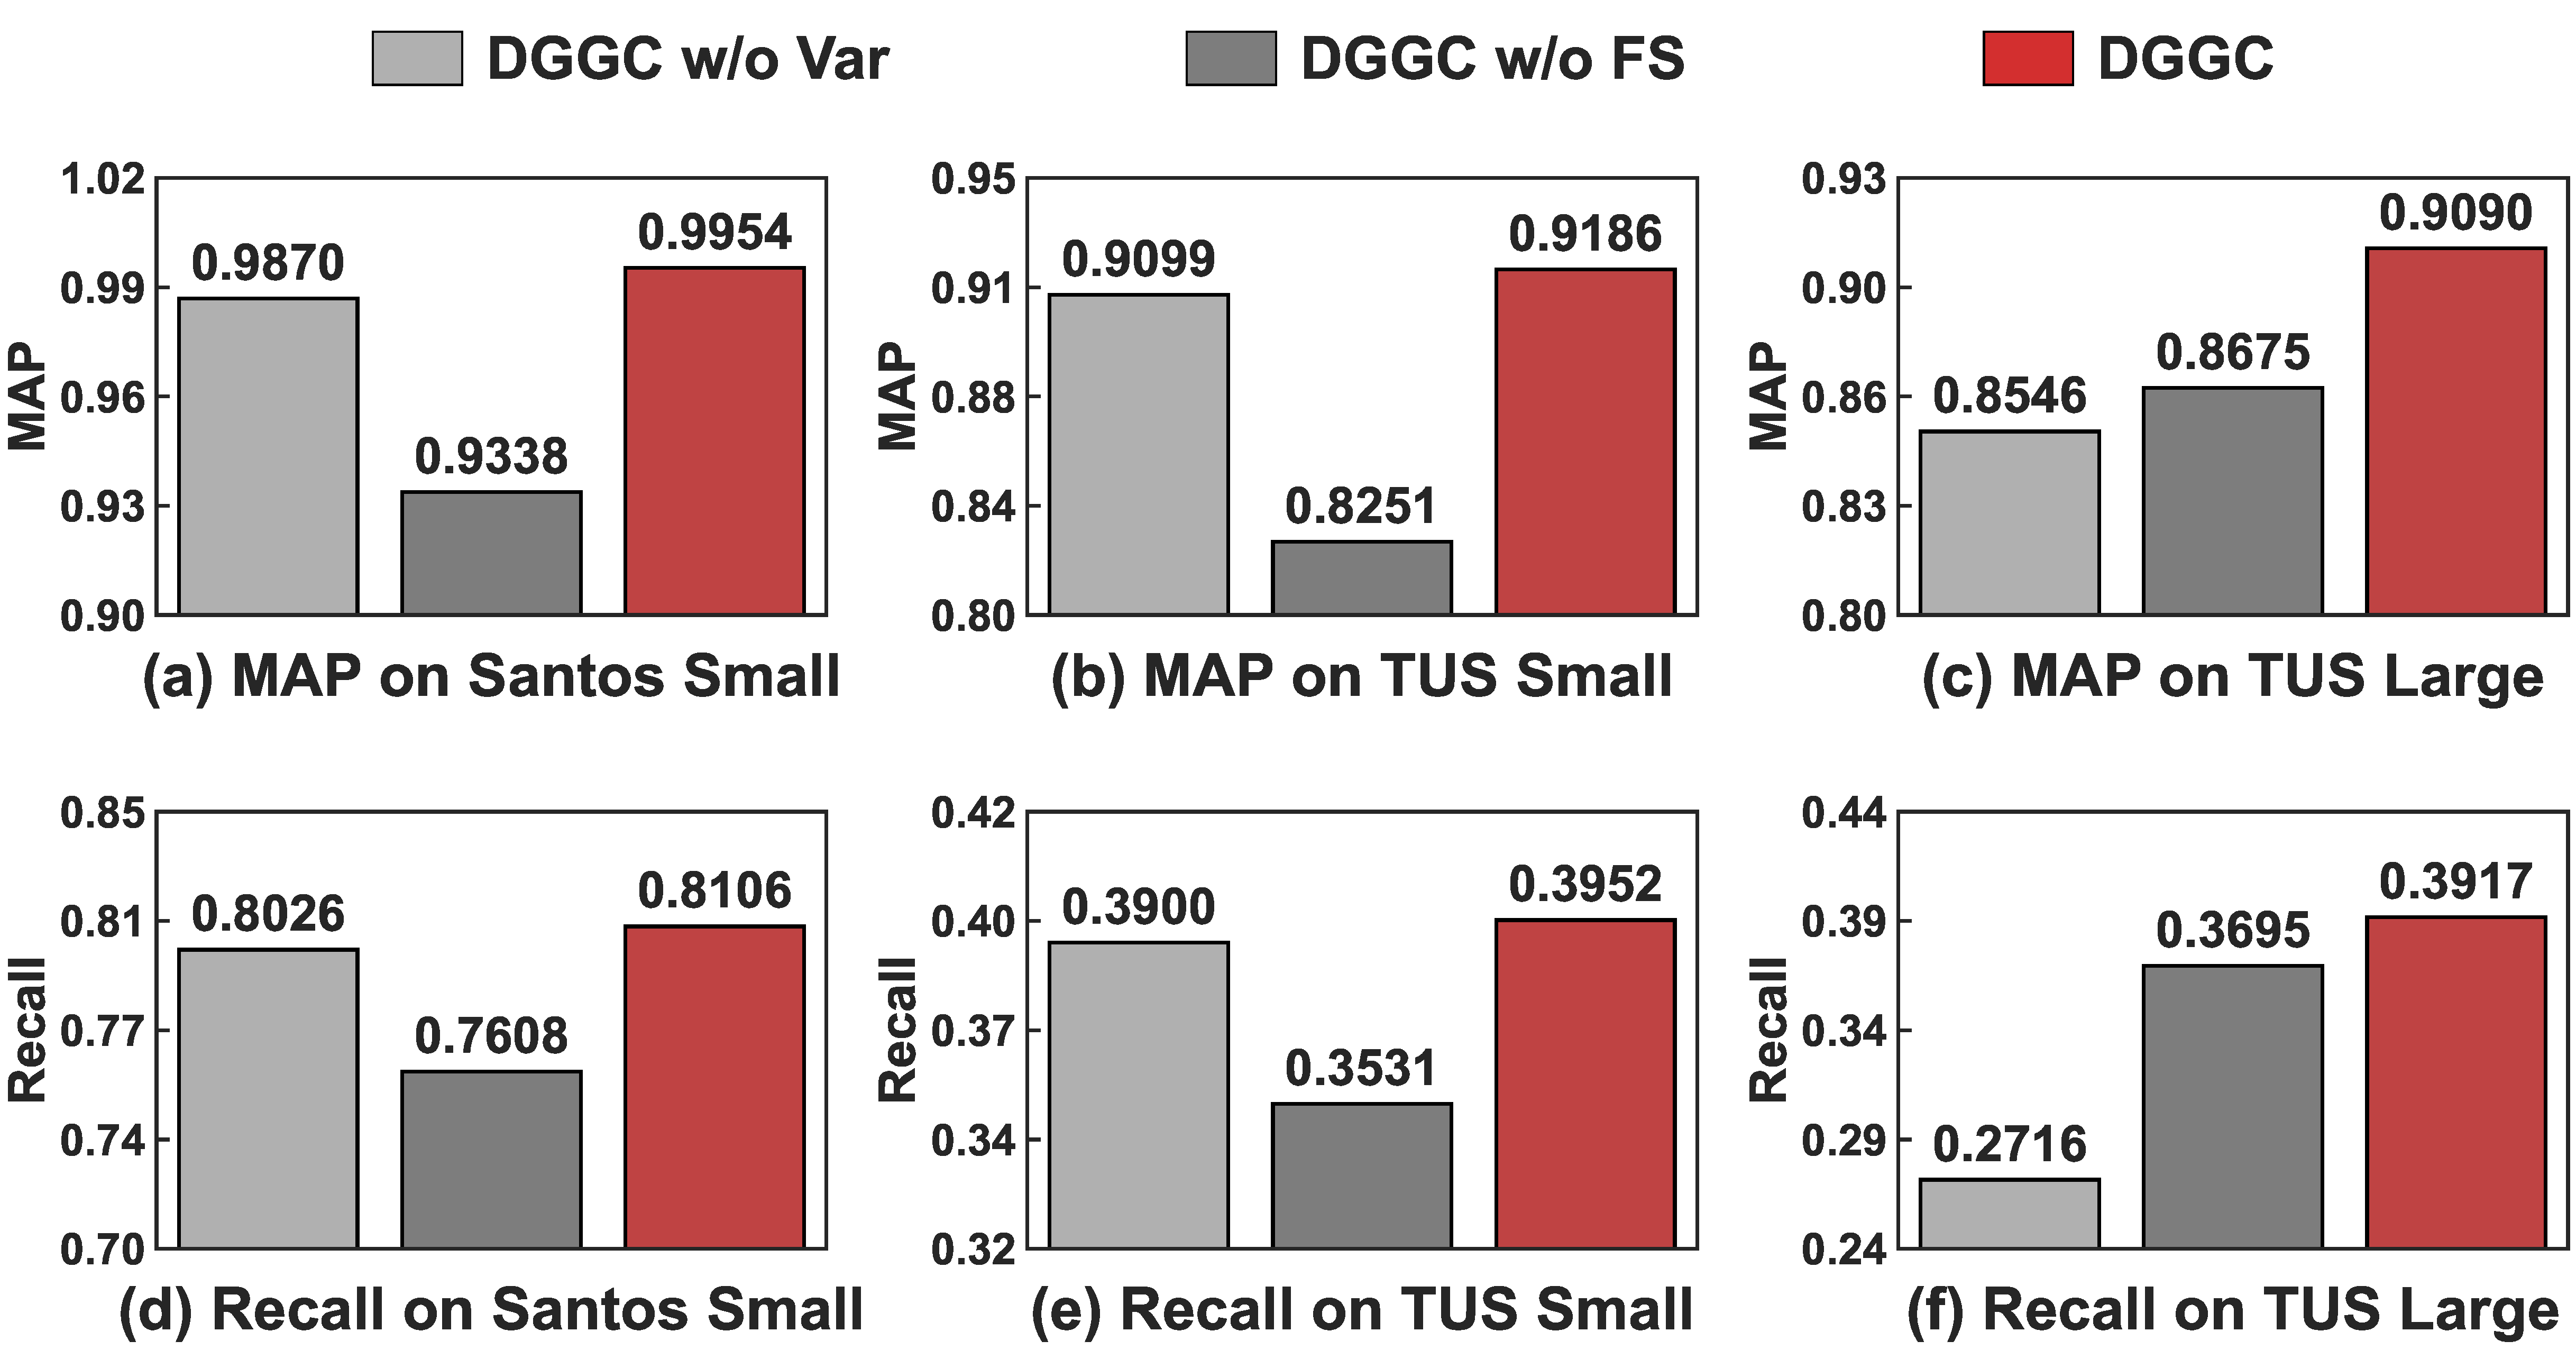
\includegraphics[width=.99\textwidth]{figure/ablation_study.pdf}
    \caption{
        {Ablation results.} 
        %The top row (a)-(c) reports the MAP@k scores, while the bottom row (d)-(f) reports the R@k  scores on Santos-Small, TUS-Small, and TUS-Large benchmarks, respectively. 
        %The red bars denote our proposed full model (DGGC (Full)). 
        %We compare it against three variants: the point embedding baseline (DGGC w/o Var), the unconstrained Gaussian variant DGGC (w/o wass), and the graph-free variant DGGC w/o FS. 
        %DGGC (Full) demonstrates consistent superiority across all metrics and datasets.
    }
    \label{fig:ablation_study}
\end{figure*}

We perform an ablation study to understand the impact of dual-granularity Gaussian embeddings, the Wasserstein-based score, and the filter-shuffle positive sample generator. We compare full DGGC with DGGC w/o FS and DGGC w/o Var, as shown in Figure~\ref{fig:ablation_study}.

DGGC consistently obtains the best results across all benchmarks. On TUS-Large, DGGC w/o Var yields a lower MAP@60 than DGGC, indicating that point-based embeddings cannot effectively model semantic specificity. For DGGC w/o FS, performance drops markedly on smaller datasets. On TUS-Small, removing the filter-shuffle mechanism reduces MAP@k from 0.9186 to 0.8251, and a similar trend appears on SANTOS-Small. This suggests that the filter-shuffle sample generator alleviates positive-sample sparsity in data-scarce environments.

\noindent\textbf{Modeling Semantic Specificity.} The degradation of DGGC w/o Var on TUS-Large shows the limitation of point embeddings in large-scale data lakes. Many candidate tables are close in the mean semantic space but differ in entity coverage or attribute granularity. DGGC introduces variance embeddings and a Wasserstein-based distance to model such semantic specificity.

\noindent\textbf{Mitigating Self-Reference Bias.} The decline of DGGC w/o FS on TUS-Small and SANTOS-Small supports the impact of self-referential bias in standard contrastive learning~\cite{robinson2021contrastive}. The filter-shuffle generator enriches training with cross-table positives and encourages the encoder to capture structural patterns beyond surface token overlap.

\noindent\textbf{Dual-Granularity Alignment.} The table-column alignment loss \(\mathcal{L}_{align}\) enforces consistency between global and local semantic views~\cite{hjelm2018learning}. This constraint prevents the table embedding from drifting due to irrelevant or noisy columns and improves representation stability.


\iffalse

\subsection{Effect of Filtering Threshold}

We also evaluate the impact of the filtering threshold $\tau$ in the Filter-Shuffle strategy (Section~\ref{sub_sec_gau}). Since our framework relies on heuristic filtering to construct training pairs, $\tau$ governs the critical trade-off between the signal-to-noise ratio (lexical reliability) and the semantic coverage (diversity) of the positive samples~\cite{dehghani2017neural}. A table pair is selected for shuffling phase only if its filtering score $f(t,t') > \tau$. The result is presented in Table \ref{eff_tau}.

As evidenced by the results in Table~\ref{eff_tau}, the performance exhibits a consistent ``rise-and-fall'' trend across all benchmarks, generating a peak in  $\tau \in [0.1, 0.2]$. The trend underscores a critical trade-off in contrastive sample selection. The initial performance gain as $\tau$ increases from $0$ to an optimal range ($0.1$–$0.2$) stems from effective noise suppression. The model with $\tau=0$ provides the training with excessive false positives from the raw retrieval output, overwhelming the model with contradictory signals. A higher threshold acts as a necessary denoiser, pruning candidates with negligible overlap to increase the prior probability of semantic relevance. The subsequent decline for $\tau > 0.5$ indicates a loss of sample diversity. An overly strict filter eliminates the heterogeneous yet semantically unionable table pairs—precisely the samples needed to combat the self-referential bias. Consequently, the model regresses to overfitting  lexical matches, failing to learn generalizable semantic representations. This validates our core design intuition: effective contrastive learning for union search should preserve a diverse positive samples to navigate the tension between signal purity and generalization capacity~\cite{chen2020simple}. The optimal $\tau$ thus balances this trade-off.

\begin{table}[t]
  \centering
  \caption{\textbf{Effect of Filtering Threshold $\tau$.}}
  \label{eff_tau}
  \begin{tabular}{c|cc|cc|cc}
    \toprule 
    {\multirow{2}{*}{$\tau$}}&\multicolumn{2}{c|}{SANTOS-Small}&\multicolumn{2}{c|}{TUS-Small}&\multicolumn{2}{c}{TUS-Large}\\
    &MAP@k&R@k&MAP@k&R@k&MAP@k&R@k\\
    \midrule
    $\tau=0$&.9491&.7681&.9601&.0769&.9091&.0507\\
    $\tau=0.1$&.9768&.7871&.9615&.0769&.9114&.0509\\
    $\tau=0.2$&.9932&.8086&.9603&.0772&.9129&.0509\\
    $\tau=0.3$&.9810&.8021&.9591&.0769&.9107&.0509\\
    $\tau=0.5$&.9744&.7933&.9589&.0767&.9090&.0506\\
    $\tau=0.7$&.9713&.7886&.9570&.0769&.9088&.0505\\
    $\tau=0.9$&.9217&.7445&.9521&.0767&.9097&.0505\\
    $\tau=1.0$&.9000&.7423&.9546&.0762&.9002&.0500\\
  \bottomrule
\end{tabular}
\end{table}
\fi

\iffalse
\subsection{Effect of Filter-Shuffle Positive Sample Generation Parameter }
\label{sec_param_analysis}

The quality of automatically mined positive pairs directly affects the
contrastive learning process  (Section~\ref{sub_sec_gau}). We therefore analyze the key factors used in the
filtering phase of the strength-aware relation map. These factors are related
to the construction of training positives rather than to the optimization of
the neural encoder itself. Specifically, the threshold on the final filtering
score \(f(t,t')\) controls the reliability of mined positive table pairs, the
structural coherence constraint \(\gamma\) specifies the minimum structural
support required for a retained pair, and the retained-neighbor number \(K\)
controls the density of the positive graph. This analysis does not aim to
identify a universal threshold. Instead, it studies how the strength-aware
relation map balances positive reliability and positive coverage across
datasets.


The quality of automatically mined positives directly affects contrastive learning  (Section~\ref{sub_sec_gau}). We therefore analyze three filtering-phase parameters of the strength-aware relation map: the threshold \(\tau\), the structural coherence constraint \(\gamma\), and the retained-neighbor number \(K\). The threshold \(\tau\) controls the minimum filtering score \(f(t,t')\), \(\gamma\) controls the minimum alignment strength \(M(t,t')\), and \(K\) limits the retained candidates for each anchor table. Table~\ref{tab:relationmap_parameter_effects} reports the three one-factor sensitivity studies.

\textbf{Effect of Filtering Threshold. }The threshold on \(f(t,t')\) directly controls positive strength. A loose
threshold preserves more positive candidates but may retain weak positives. In
contrast, an overly strict threshold improves the reliability of retained
pairs but may reduce positive coverage. As shown in
Table~\ref{tab:relationmap_parameter_effects}(a), SANTOS-SMALL performs best around
\(\tau=0.65\), where MAP@k reaches 0.9912 and R@k reaches 0.4025. Increasing
the threshold to \(\tau=0.85\) reduces MAP@k to 0.9657 and R@k to 0.3808.
TUS-SMALL is relatively stable across the tested range, with MAP@k varying
only from 0.9569 to 0.9577. TUS-LARGE shows a clearer rise-and-fall pattern.
MAP@k improves from 0.8826 at \(\tau=0.60\) to 0.8975 at \(\tau=0.75\), but
drops to 0.8794 at \(\tau=0.85\). This result indicates that the filtering
threshold should remove weak positives without making the positive graph
overly sparse.

The corresponding relation-map statistics further explain this pattern. On
SANTOS-SMALL, increasing the threshold from 0.65 to 0.85 reduces the graph from
3844 edges with average degree 9.31 to 1426 edges with average degree 5.73.
Meanwhile, the mean matched count and mean coverage increase from 7.35 and
0.832 to 8.91 and 0.973. This suggests that the performance drop is caused by
insufficient positive coverage rather than by weaker retained pairs.
TUS-SMALL remains stable because the graph still keeps 4860 edges and average
degree 5.51 at \(\tau=0.85\), while the matched count and coverage increase to
8.16 and 0.861. On TUS-LARGE, moderate filtering is more effective. MAP@k
improves from 0.8826 at \(\tau=0.60\) to 0.8975 at \(\tau=0.75\), but drops to
0.8794 when the graph shrinks to 8749 edges and average degree 4.62 at
\(\tau=0.85\). These results show that the threshold on \(f(t,t')\) should
increase positive reliability while preserving sufficient graph connectivity.

\textbf{Effect of Structural Coherence Constraint \(\gamma\). }The structural coherence constraint \(\gamma\) controls the minimum alignment
strength \(M(t,t')\) required for a table pair to be retained.As shown in
Table~\ref{tab:relationmap_parameter_effects}(b), SANTOS-SMALL is stable from
\(\gamma=0.05\) to \(\gamma=0.30\), where MAP@k remains 0.9946 and R@k remains
around 0.7980. TUS-SMALL is also insensitive to this constraint in the tested
range, with MAP@k fixed at 0.9575. TUS-LARGE is more sensitive. MAP@k reaches
0.9007 at \(\gamma=0.10\), remains close at \(\gamma=0.15\), and drops to
0.8892 at \(\gamma=0.30\). This trend supports the subset-based interpretation
of semantic unionability, where useful positive pairs may be removed if the
structural constraint is too strict.

This effect is mainly reflected in graph sparsity. On SANTOS-SMALL and
TUS-SMALL, the graph statistics change only slightly across the tested range,
which explains the stable retrieval scores. On TUS-LARGE, relaxed constraints
\(\gamma=0.05\), \(\gamma=0.10\), and \(\gamma=0.15\) produce the same graph
statistics, with 29697 edges, average degree 8.00, mean matched count 6.56,
and mean coverage 0.737. Increasing \(\gamma\) to 0.30 and 0.50 reduces the
graph to 28957 and 26857 edges, respectively, and leads to lower MAP@k. This
result is consistent with the semantic unionability definition. Valid
positives do not necessarily require full schema coverage, and overly strict
structural constraints may remove useful subset-based matches.
\textbf{Effect of Positive-Neighbor Width \(K\). }The retained-neighbor number \(K\) controls the width of the positive graph. A
very small \(K\) may discard useful positives, while a very large \(K\), or
using all retained neighbors, does not consistently improve retrieval. As
shown in Table~\ref{tab:relationmap_parameter_effects}(c), SANTOS-SMALL benefits from
increasing \(K\) from 4 to 16, with MAP@k improving from 0.9874 to 0.9994.
However, increasing \(K\) to 80 or using all retained neighbors reduces MAP@k
to 0.9946. TUS-SMALL saturates once \(K\geq 8\), where MAP@k remains 0.9575.
TUS-LARGE achieves its best MAP@k at \(K=12\), reaching 0.8943. Larger
neighborhoods do not further improve performance. Therefore, \(K\) should be
treated as a bounded-neighborhood parameter rather than a quantity to maximize.

The graph statistics support this conclusion. On SANTOS-SMALL, increasing
\(K\) from 4 to 16 expands the graph from 1471 edges with average degree 3.60
to 3612 edges with average degree 8.83, which improves MAP@k. Increasing
\(K\) to 80 further expands the graph to 3768 edges, but no longer improves
performance. TUS-SMALL saturates after \(K=8\), where the graph reaches 9913
edges and average degree 7.76. TUS-LARGE follows a similar pattern. Increasing
\(K\) from 4 to 12 improves positive coverage and MAP@k, while larger values
produce nearly unchanged graph statistics. These results indicate that too
small a neighborhood loses positive coverage, whereas too large a neighborhood
mainly adds redundant or weaker positives.




\begin{table}[t]
\centering
\caption{\textbf{Effect of strength-aware relation map parameters.}
The table reports MAP@k and R@k on SANTOS-SMALL, TUS-SMALL, and TUS-LARGE.
Panels (a)--(c) correspond to the filtering threshold, structural coherence constraint, and positive-neighbor width, respectively.}
\label{tab:relationmap_parameter_effects}
\footnotesize
\setlength{\tabcolsep}{4pt}
\renewcommand{\arraystretch}{0.92}
\begin{tabular}{l|cc|cc|cc}
\toprule
\multirow{2}{*}{Setting}
& \multicolumn{2}{c|}{SANTOS-SMALL}
& \multicolumn{2}{c|}{TUS-SMALL}
& \multicolumn{2}{c}{TUS-LARGE} \\
& MAP@k & R@k & MAP@k & R@k & MAP@k & R@k \\
\midrule
\multicolumn{7}{l}{\textbf{(a) Effect of Filtering Threshold  \(\tau\)}} \\
\midrule
\(\tau=0.60\) & .9904 & .4010 & .9574 & .3769 & .8826 & .2079 \\
\(\tau=0.65\) & .9912 & .4025 & .9577 & .3769 & .8898 & .2086 \\
\(\tau=0.70\) & .9846 & .3980 & .9575 & .3800 & .8924 & .2109 \\
\(\tau=0.75\) & .9780 & .3927 & .9575 & .3801 & .8975 & .2110 \\
\(\tau=0.80\) & .9720 & .3860 & .9569 & .3774 & .8890 & .2090 \\
\(\tau=0.85\) & .9657 & .3808 & .9571 & .3771 & .8794 & .2065 \\
\midrule
\multicolumn{7}{l}{\textbf{(b) Effect of Structural Coherence Constraint \(\gamma\)}} \\
\midrule
\(\gamma=0.05\) & .9946 & .7980 & .9575 & .3569 & .9000 & .2120 \\
\(\gamma=0.10\) & .9946 & .7980 & .9575 & .3569 & .9007 & .2123 \\
\(\gamma=0.15\) & .9946 & .7980 & .9575 & .3569 & .9004 & .2122 \\
\(\gamma=0.30\) & .9946 & .7981 & .9575 & .3564 & .8892 & .2108 \\
\(\gamma=0.50\) & .9924 & .7969 & .9575 & .3568 & .8921 & .2110 \\
\midrule
\multicolumn{7}{l}{\textbf{(c) Effect of Positive-Neighbor Width \(K\)}} \\
\midrule
\(K=4\)   & .9874 & .7890 & .9570 & .3564 & .8859 & .2078 \\
\(K=8\)   & .9920 & .7950 & .9575 & .3569 & .8910 & .2109 \\
\(K=12\)  & .9964 & .8007 & .9575 & .3569 & .8943 & .2110 \\
\(K=16\)  & .9994 & .8026 & .9575 & .3569 & .8935 & .2108 \\
\(K=80\)  & .9946 & .7980 & .9575 & .3569 & .8926 & .2105 \\
\(K=\mathrm{all}\) & .9946 & .7980 & .9575 & .3569 & .8927 & .2105 \\
\bottomrule
\end{tabular}
\end{table}
Overall, the statistics show that performance depends on the balance between
positive strength and positive coverage. Stricter filtering usually increases
matched count or coverage, but if it sharply reduces edges and average degree,
the positive graph becomes too sparse. Conversely, a denser graph is not
always better, since excessive neighbors may introduce redundant or weak
positives. Therefore, the best relation map is neither the strictest nor the
densest one, but the one that preserves sufficient reliable positive edges for
contrastive learning.
\fi

\subsection{Effect of Filter-Shuffle Positive Sample Generation Parameters}
\label{sec_param_analysis}

The quality of automatically mined positives directly affects contrastive learning. We therefore analyze three filtering-phase parameters of the strength-aware relation map: the filtering threshold \(\tau\), the structural coherence constraint \(\gamma\), and the retained-neighbor width \(K\). The threshold \(\tau\) controls the minimum filtering score \(f(t,t')\), \(\gamma\) controls the minimum alignment strength \(M(t,t')\), and \(K\) limits the retained candidates for each anchor table. Table~\ref{tab:relationmap_parameter_effects} reports the one-factor sensitivity results.

\noindent\textbf{Effect of \(\tau\).}
The filtering threshold controls the trade-off between positive reliability and positive coverage. A loose threshold preserves more candidates but may retain weak positives, whereas an overly strict threshold makes the positive graph sparse. As shown in Table~\ref{tab:relationmap_parameter_effects}(a), SANTOS-SMALL performs best around \(\tau=0.65\), while TUS-LARGE reaches its best MAP@k at \(\tau=0.75\). The performance drop at higher thresholds indicates that excessive filtering removes useful cross-table positives.

\noindent\textbf{Effect of \(\gamma\).}
The structural coherence constraint controls the minimum alignment strength required for a retained pair. Table~\ref{tab:relationmap_parameter_effects}(b) shows that SANTOS-SMALL and TUS-SMALL are relatively stable across the tested range, whereas TUS-LARGE is more sensitive. This result is consistent with the subset-based definition of semantic unionability: valid positives do not necessarily require full schema coverage, and overly strict structural constraints may remove useful partial matches.

\noindent\textbf{Effect of \(K\).}
The retained-neighbor width determines the density of the positive graph. As shown in Table~\ref{tab:relationmap_parameter_effects}(c), increasing \(K\) improves positive coverage at first, but larger neighborhoods do not consistently improve retrieval performance. This suggests that \(K\) should be treated as a bounded-neighborhood parameter rather than a quantity to maximize.

\begin{table}[t]
\centering
\caption{\textbf{Effect of filter-shuffle positive sample generation parameters.}
The table reports MAP@k and R@k on SANTOS-SMALL, TUS-SMALL, and TUS-LARGE.}
\label{tab:relationmap_parameter_effects}
\footnotesize
% \setlength{\tabcolsep}{3.5pt}
% \renewcommand{\arraystretch}{0.9}
\resizebox{\columnwidth}{!}{%
\begin{tabular}{l|cc|cc|cc}
\toprule
\multirow{2}{*}{Setting}
& \multicolumn{2}{c|}{SANTOS-SMALL}
& \multicolumn{2}{c|}{TUS-SMALL}
& \multicolumn{2}{c}{TUS-LARGE} \\
& MAP@k & R@k & MAP@k & R@k & MAP@k & R@k \\
\midrule
\multicolumn{7}{l}{\textbf{(a) Filtering threshold \(\tau\)}} \\
\midrule
\(\tau=0.60\) & .9904 & .4010 & .9574 & .3769 & .8826 & .2079 \\
\(\tau=0.65\) & .9912 & .4025 & .9577 & .3769 & .8898 & .2086 \\
\(\tau=0.70\) & .9846 & .3980 & .9575 & .3800 & .8924 & .2109 \\
\(\tau=0.75\) & .9780 & .3927 & .9575 & .3801 & .8975 & .2110 \\
\(\tau=0.80\) & .9720 & .3860 & .9569 & .3774 & .8890 & .2090 \\
\(\tau=0.85\) & .9657 & .3808 & .9571 & .3771 & .8794 & .2065 \\
\midrule
\multicolumn{7}{l}{\textbf{(b) Structural coherence \(\gamma\)}} \\
\midrule
\(\gamma=0.05\) & .9946 & .7980 & .9575 & .3569 & .9000 & .2120 \\
\(\gamma=0.10\) & .9946 & .7980 & .9575 & .3569 & .9007 & .2123 \\
\(\gamma=0.15\) & .9946 & .7980 & .9575 & .3569 & .9004 & .2122 \\
\(\gamma=0.30\) & .9946 & .7981 & .9575 & .3564 & .8892 & .2108 \\
\(\gamma=0.50\) & .9924 & .7969 & .9575 & .3568 & .8921 & .2110 \\
\midrule
\multicolumn{7}{l}{\textbf{(c) Positive-neighbor width \(K\)}} \\
\midrule
\(K=4\)   & .9874 & .7890 & .9570 & .3564 & .8859 & .2078 \\
\(K=8\)   & .9920 & .7950 & .9575 & .3569 & .8910 & .2109 \\
\(K=12\)  & .9964 & .8007 & .9575 & .3569 & .8943 & .2110 \\
\(K=16\)  & .9994 & .8026 & .9575 & .3569 & .8935 & .2108 \\
\(K=80\)  & .9946 & .7980 & .9575 & .3569 & .8926 & .2105 \\
\(K=\mathrm{all}\) & .9946 & .7980 & .9575 & .3569 & .8927 & .2105 \\
\bottomrule
\end{tabular}%
}%
\end{table}

Overall, the results show that the best relation map is neither the strictest nor the densest one. DGGC benefits from retaining sufficiently reliable positive edges while preserving enough graph connectivity for contrastive learning.

\iffalse
\subsection{Effect of Loss Function Parameter}
We further investigate the sensitivity of DGGC to the hyper-parameter $\lambda$, which balances the mean embedding and variance embedding in the loss function (Eq.~\eqref{eq_gs}). We vary $\lambda$ within the range of $[0,2]$ to assess its impact on retrieval stability in Table \ref{eff_lam}. 

As evidenced by the results in Table~\ref{eff_lam}, incorporating the variance penalty ($\lambda > 0$) consistently yields superior performance compared to the only mean embeddings ($\lambda = 0$), validating that our distribution-based representation effectively provides semantic specificity distribution for effective table union search.

The optimal parameter $\lambda$ for balancing the mean and variance terms in the loss function varies significantly across benchmark, reflecting their distinct data characteristics. On SANTOS-Small, which contains tables with dense records, performance peaks at $\lambda=0.30$. This indicates a need to moderately weigh the variance, ensuring that alignment in semantic specificity complements the primary similarity signal from the mean embeddings. In contrast, TUS-Large, which is characterized by high column dimensionality but sparse rows, requires a substantially stronger $\lambda=1.60$. With such high-dimensional, low-sample-size nature, emphasizing the variance term is crucial to enforce consistency in semantic specificity, thereby suppressing overfitting to spurious correlations in the mean embeddings. Conversely, TUS-Small, with its cleaner and more consistent semantic patterns, achieves optimal results with a minimal $\lambda=0.02$. Here, excessive focus on specificity alignment ($\lambda\geq 0.20$) leads to over-regularization and performance degradation. These results demonstrate that $\lambda$ effectively modulates the trade-off between general semantic similarity (via mean embeddings) and consistency in semantic specificity (via variance embeddings). The required balance is dataset-dependent: sparse, heterogeneous data necessitates strong specificity regularization, while compact, homogeneous data relies more on traditional semantic similarity.

\begin{table}[t]
  \centering
  \caption{Effect of Loss Function Parameter $\lambda$.}
  \label{eff_lam}
  \begin{tabular}{c|cc|cc|cc}
    \toprule 
    {\multirow{2}{*}{$\lambda$}}&\multicolumn{2}{c|}{SANTOS-Small}&\multicolumn{2}{c|}{TUS-Small}&\multicolumn{2}{c}{TUS-Large}\\
    &MAP@k&R@k&MAP@k&R@k&MAP@k&R@k\\
    \midrule
    $\lambda=0$&.9844&.8013&.9601&.3769&.9072&.2545\\
    $\lambda=0.02$&.9876&.8062&.9615&.3769&.9072&.2546\\
    $\lambda=0.10$&.9891&.8046&.9603&.3772&.9082&.2506\\
    $\lambda=0.20$&.9875&.8026&.9591&.3769&.9061&.2502\\
    $\lambda=0.30$&.9918&.8066&.9589&.3767&.9082&.2507\\
    $\lambda=0.40$&.9890&.8046&.9570&.3769&.9100&.2507\\
    $\lambda=1.00$&.9889&.8041&.9521&.3767&.9105&.2507\\
    $\lambda=1.60$&.9903&.8056&.9546&.3762&.9118&.2508\\
    $\lambda=2.00$&.9896&.8052&.9528&.3768&.9111&.2508\\
  \bottomrule
\end{tabular}
\end{table}
\fi
\subsection{Effect of Loss Function Parameter}
\label{sec_lambda}

We further investigate the sensitivity of DGGC to the hyperparameter \(\lambda\), which balances the mean embedding and variance embedding in the loss function (Eq.~\eqref{eq_gs}). We vary \(\lambda\) within \([0,2]\) and report its impact on retrieval stability in Table~\ref{eff_lam}.

\begin{table}[!htbp]
  \centering
  \caption{Effect of loss function parameter \(\lambda\).}
  \label{eff_lam}
  \footnotesize
  % \setlength{\tabcolsep}{2.8pt}
  % \renewcommand{\arraystretch}{0.88}
  \resizebox{\columnwidth}{!}{%
  \begin{tabular}{c|cc|cc|cc}
    \toprule 
    \multirow{2}{*}{\(\lambda\)}
    & \multicolumn{2}{c|}{SANTOS-Small}
    & \multicolumn{2}{c|}{TUS-Small}
    & \multicolumn{2}{c}{TUS-Large} \\
    & MAP@k & R@k & MAP@k & R@k & MAP@k & R@k \\
    \midrule
    0    & .9844 & .8013 & .9601 & .0769 & .9072 & .0545 \\
    .02  & .9876 & .8062 & .9615 & .0769 & .9072 & .0546 \\
    .10  & .9891 & .8046 & .9603 & .0772 & .9082 & .0506 \\
    .20  & .9875 & .8026 & .9591 & .0769 & .9061 & .0502 \\
    .30  & .9918 & .8066 & .9589 & .0767 & .9082 & .0507 \\
    .40  & .9890 & .8046 & .9570 & .0769 & .9100 & .0507 \\
    1.00 & .9889 & .8041 & .9521 & .0767 & .9105 & .0507 \\
    1.60 & .9903 & .8056 & .9546 & .0762 & .9118 & .0508 \\
    2.00 & .9896 & .8052 & .9528 & .0768 & .9111 & .0508 \\
    \bottomrule
  \end{tabular}%
  }%
\end{table}

As shown in Table~\ref{eff_lam}, incorporating the variance penalty \((\lambda>0)\) generally yields better performance than using mean-only embeddings \((\lambda=0)\), validating that the distribution-based representation captures semantic specificity for table union search. The optimal value of \(\lambda\) varies across benchmarks, reflecting their different data characteristics. SANTOS-Small reaches the best performance at \(\lambda=0.30\), indicating that a moderate variance weight complements the primary similarity signal from mean embeddings. TUS-Large, which has higher column dimensionality and sparser rows, benefits from a stronger weight \((\lambda=1.60)\), since emphasizing variance helps enforce semantic specificity and suppress spurious correlations in mean embeddings. In contrast, TUS-Small achieves the best result with a small weight \((\lambda=0.02)\), while larger values cause over-regularization. These results show that \(\lambda\) modulates the trade-off between general semantic similarity and specificity consistency, and the required balance depends on dataset scale and heterogeneity.

\subsection{Efficiency of DGGC}
We evaluate the computational efficiency and scalability of our framework on datasets ranging from small benchmarks to a one-million-table data lake. Table~\ref{tab:scalability} reports the index construction time and average retrieval latency. %Our evaluation incorporates the full context window (up to 512 tokens) to assess system robustness under maximum information load.
\begin{table}[!htbp]
  \centering
  \caption{Response time of index construction and table union search}
  \label{tab:scalability}
  
  \resizebox{\columnwidth}{!}{%
  \begin{tabular}{c|c|cc}
    \toprule
    \multirow{2}{*}{Corpus} & \multirow{2}{*}{\#Tabs}& \multicolumn{2}{c}{Time} \\
     & & Index (s) & Search (ms) \\
    \midrule
    SANTOS Small & 550 & 0.0001& 0.002\\
    TUS Small & 1,526 & 0.0004& 0.005\\
    TUS Large & 5,044 & 0.0013& 0.006 \\
    SANTOS Large & 11,065 & 0.0029& 0.041 \\
    WDC (1M)& 1,000,000 & 0.2154& 3.819 \\
    \bottomrule
  \end{tabular}%
  }%
\end{table}

The empirical results demonstrate a high degree of scalability for online table union search. Even with full-context serialization, the encoding complexity remains bounded by the constant model overhead rather than data volume. Specifically, the encoding time remains stable at approximately 6.6 ms per column at most. Furthermore, the index construction of {Flat Vector Index} for one million tables completes in merely 0.215 seconds. On the largest dataset (WDC Sample, 1M tables), the system maintains an average latency of {3.82 ms}. The FAISS Flat Index maintains millisecond-level retrieval latency in our setting ~\cite{johnson2019billion,aumuller2020ann}.

\subsection{Case Study}
\label{app:case_study}
\iffalse
We further provide a case study on the ``Wholesale Markets'' domain to examine how DGGC handles lexical overlap and semantic specificity. DGGC w/o Var retrieves a restaurant and retail table with high lexical overlap, while DGGC retrieves a true positive table about public wholesale markets. The training dynamics show that variance embeddings help reduce the influence of hard negative candidates whose mean embeddings are close to the query but whose semantic specificity is inconsistent. The full case study, including the returned tables and training curves, is provided in Appendix~\ref{app:case_study}.
\fi
To intuitively understand the superiority of DGGC in handling semantic specificity in tables, we provide a case study focusing on the tables about ``Wholesale Markets'', a domain where heavy lexical overlap frequently impacts the performance of union search. Figure \ref{fig:casestudy} presents the query table and the union search results returned by DGGC and DGGC w/o Var. Figure \ref{fig:case_study_epoch} shows the MAP of all queries and the cosine similarity between the mean embedding of the query table in the case study and its hard negative sample embedding as the epoch increases.

\begin{figure}[!htpb]
    \centering
    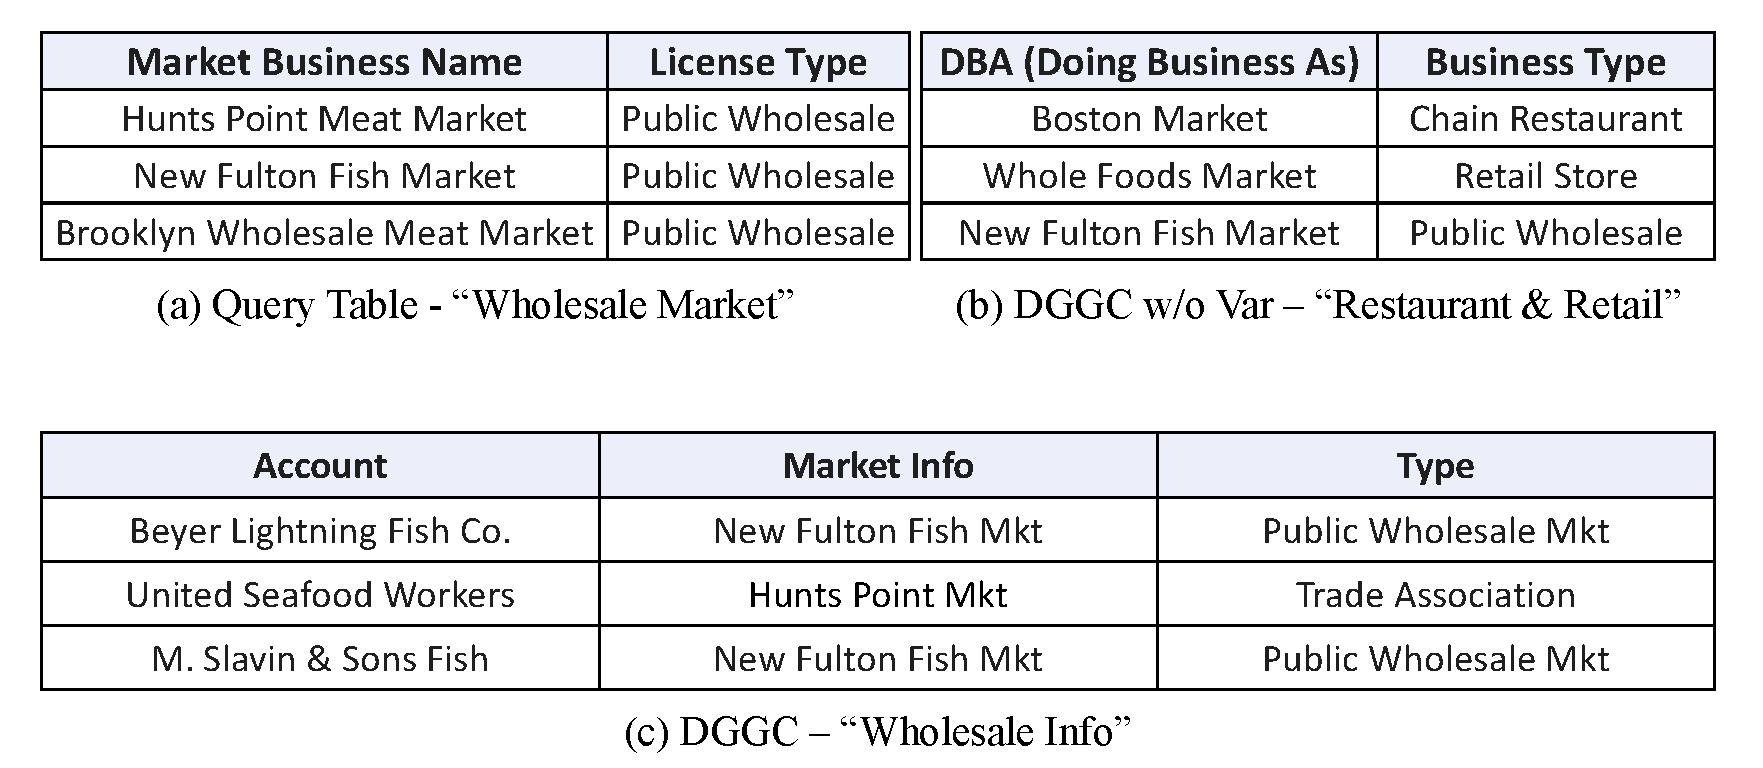
\includegraphics[width=\columnwidth]{figure/case_study.pdf}
    \caption{A case study of table union search: (a) The query table about ``Wholesale Markets''; (b) The returned table of DGGC w/o Var, which is a restaurant \& retail table due to its high lexical overlap with the query table (e.g., ``Market'', ``Type''); (c) The returned table of DGGC, which is a true positive containing markets with public wholesale type.}
    \label{fig:casestudy}
\end{figure}

As illustrated in Figure \ref{fig:casestudy} and Figure \ref{fig:case_study_epoch}, DGGC w/o Var retrieves a ``Restaurant \& Retail'' table, which is misled by severe value-level lexical overlap (estimated Jaccard similarity $\approx 0.42$ over normalized value tokens). The overlapping strings, such as ``Hunts Point Meat Market'' vs. ``Boston Market'' and ``License Type'' vs. ``Business Type'', create a high similarity between the two tables. At Epoch 1, the cosine similarity between the query table and this hard negative sample is notably high at 0.982. However, as training progresses, this similarity significantly drops to 0.2138 by Epoch 30. The overall MAP@k of DGGC w/o Var reaches its peak at Epoch 2 but subsequently begins to decline. This deterioration can be attributed to the model's neglect of semantic specificity due to the absence of a variance constraint. As a result, the model overfits to superficial lexical overlap, leading to a gradual decrease in MAP@k performance, which falls from 0.9346 to 0.7054.

\begin{figure*}[t]
    \centering
    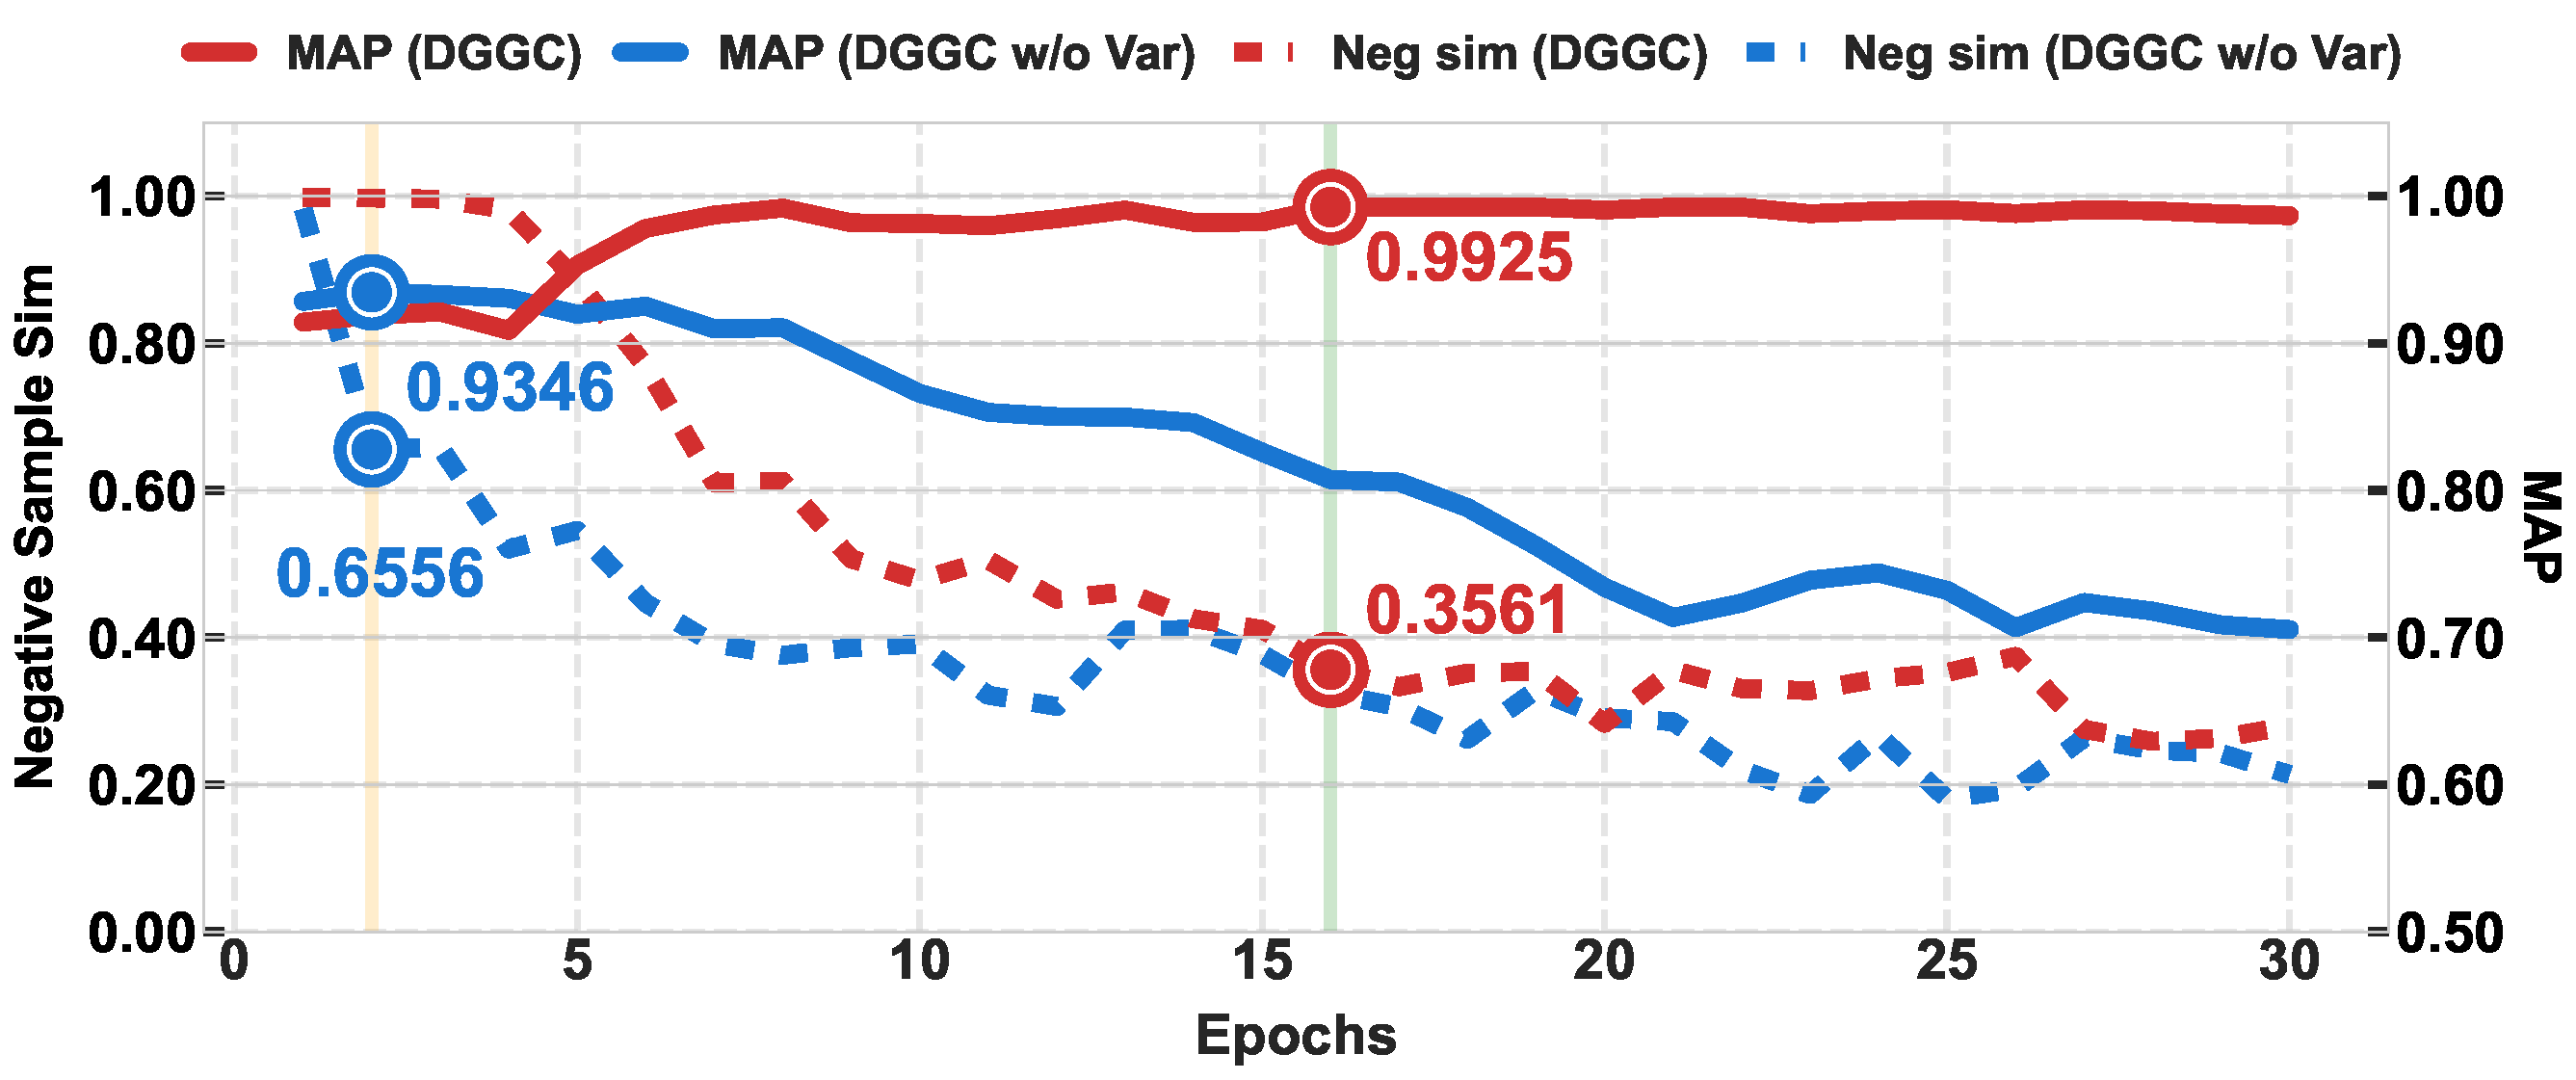
\includegraphics[width=\textwidth]{figure/case_study_epoch.pdf}
    \caption{The trend of cosine similarity between the query table and the hard negative sample, together with the total MAP, as the training epoch changes for DGGC w/o Var and DGGC. The light orange and light green vertical lines denote the epochs where the respective models achieve their optimal MAP performance.}
    \label{fig:case_study_epoch}
\end{figure*}

In contrast, the DGGC model, which incorporates variance embeddings to account for semantic specificity, effectively captures the inconsistency in table semantics illustrated in Figure \ref{fig:casestudy} (a) and (b). While both tables pertain to market entities, the query table emphasizes public wholesale markets, whereas Figure \ref{fig:casestudy} (b) focuses on more general restaurant and retail contexts. The variance embedding in the loss function sensitively detects this mismatch. During training, the variance penalty term $\lambda\|\sigma_q-\sigma_n\|_2^2$ lowers the compatibility score of candidates with inconsistent semantic specificity, even when their mean embeddings are close to the query. As a result, DGGC significantly reduces the cosine similarity between the query table and the hard negative sample from 0.9977 to 0.3561, corresponding to a 64.3\% decrease, while maintaining robust global performance, with MAP@k peaking at 0.9925. This qualitative result validates that introducing the variance constraint enables the model to distinguish genuine semantic alignment \cite{karpukhin2020dense} from superficial lexical similarity \cite{robertson2009probabilistic}, which is critical for effective retrieval in real-world data lakes.

\section{Conclusion}
\label{cld}
In this paper, we proposed DGGC, which enhances table union search through dual-granularity Gaussian learning,
and a filter-shuffle sample generator. Our key insight is that by 
exploiting semantic specificity by Gaussian learning over both tables and columns and the filter-shuffle sample generator significantly mitigates the self-referential bias of contrastive learning methods. Experimental results demonstrate the Gaussian features learned from tables and columns can provide robust unionability score and improve the table union search models.


% COLING 2027 requires this section after the conclusion and before references.
% The existing future-work sentence is reused verbatim; no scientific wording is changed.
\section{Limitations}
Future work might investigate more
sophisticated data lake such as dynamic table corpus or tables contain numerical information.


\paragraph*{Supplemental Material Statement.}
The anonymous supplemental package contains source code, configuration files,
preprocessing and evaluation scripts, and selected result CSV files corresponding
to the experimental tables in the paper. Public benchmark datasets are not
redistributed; the package provides the expected directory structure and
preprocessing instructions. If accepted, the package can be released in a public repository with a persistent archive.

\bibliography{references}

\appendix
\section{Baseline Details}
The details of our baselines are listed as follows:
\begin{itemize}
    \item D$^3$L \cite{bogatu2020dataset}  addresses the problem of finding related tables in data lakes by constructing a comprehensive similarity framework that utilizes multi-dimensional attributes such as column names, value overlap, and formatting features.  
    \item Sherlock \cite{hulsebos2019sherlock}  is a feature-based representation learning method that aggregates various micro-features, such as character embeddings, character distributions, and global table statistics, to map data columns into compact embedding vectors for semantic type detection. 
    \item SATO \cite{zhang2019sato} extends Sherlock by integrating an LDA topic model to explicitly capture global table context information, thereby performing multi-column prediction to significantly improve the robustness of semantic type detection. 
    \item SANTOS \cite{khatiwada2023santos} introduces a relationship-based approach for semantic table union search that goes beyond content matching by leveraging external and self-curated knowledge bases to infer deep semantic associations between columns.  
    \item TAPAS \cite{herzig2020tapas} extends the BERT architecture for tabular data by incorporating row and column position embeddings and utilizing a masked language modeling objective on flattened tables to achieve weakly supervised table parsing.  
    \item Doduo \cite{jiang2024doduo} builds upon a Transformer-based serialized table representation, employing a multi-task learning objective to simultaneously predict column types and column relations, thus facilitating knowledge sharing and complementarity between different semantic tasks.  
    \item Starmie \cite{fan2022semantics} presents a contrastive learning framework to generate contextualized column embeddings, utilizing serialized table content and a multi-column attention mechanism to effectively capture inter-column dependencies for optimizing table union search. 
    \item LIFTus \cite{qiu2025liftus} proposes an adaptive multi-aspect representation learning architecture that fuses linguistic features from pre-trained language models (PLMs), character-level patterns, and numerical distributions via a hierarchical cross-attention mechanism to handle heterogeneous data. 

    \iffalse
    \item w/o variance is our baseline encoder that only uses a deterministic point vector as the output of the encoder in the training process. This is DGGC (Full) without the distributional uncertainty modeling. 
    \item w/o wass is our distributional variant that utilizes the Gaussian embedding but ignores the geometric penalty in the training process. This is DGGC (Full) without the Wasserstein distance regularization. 
    \item w/o real pos is our unsupervised baseline that only uses single-table augmentation views as positive pairs in the training process. This is w/o variance without the relation-guided positive sampling. 



    \item DGGC (only header pos) is our modality variant that only uses schema information as the input of the encoder in the training process. This is DGGC (Full) without the data content information. 
    \item DGGC (only data pos) is our modality variant that only uses cell values as the input of the encoder in the training process. This is DGGC (Full) without the schema context information. 
    \item DGGC (Full) is our complete framework that utilizes both relation-guided sampling and Wasserstein distribution constraints in the training process. This is the optimal configuration incorporating all proposed components. 
    \fi

\end{itemize}

\iffalse
\end{itemize}
\section{Case Study}
\label{app:case_study}
\begin{figure}
    \centering
  
    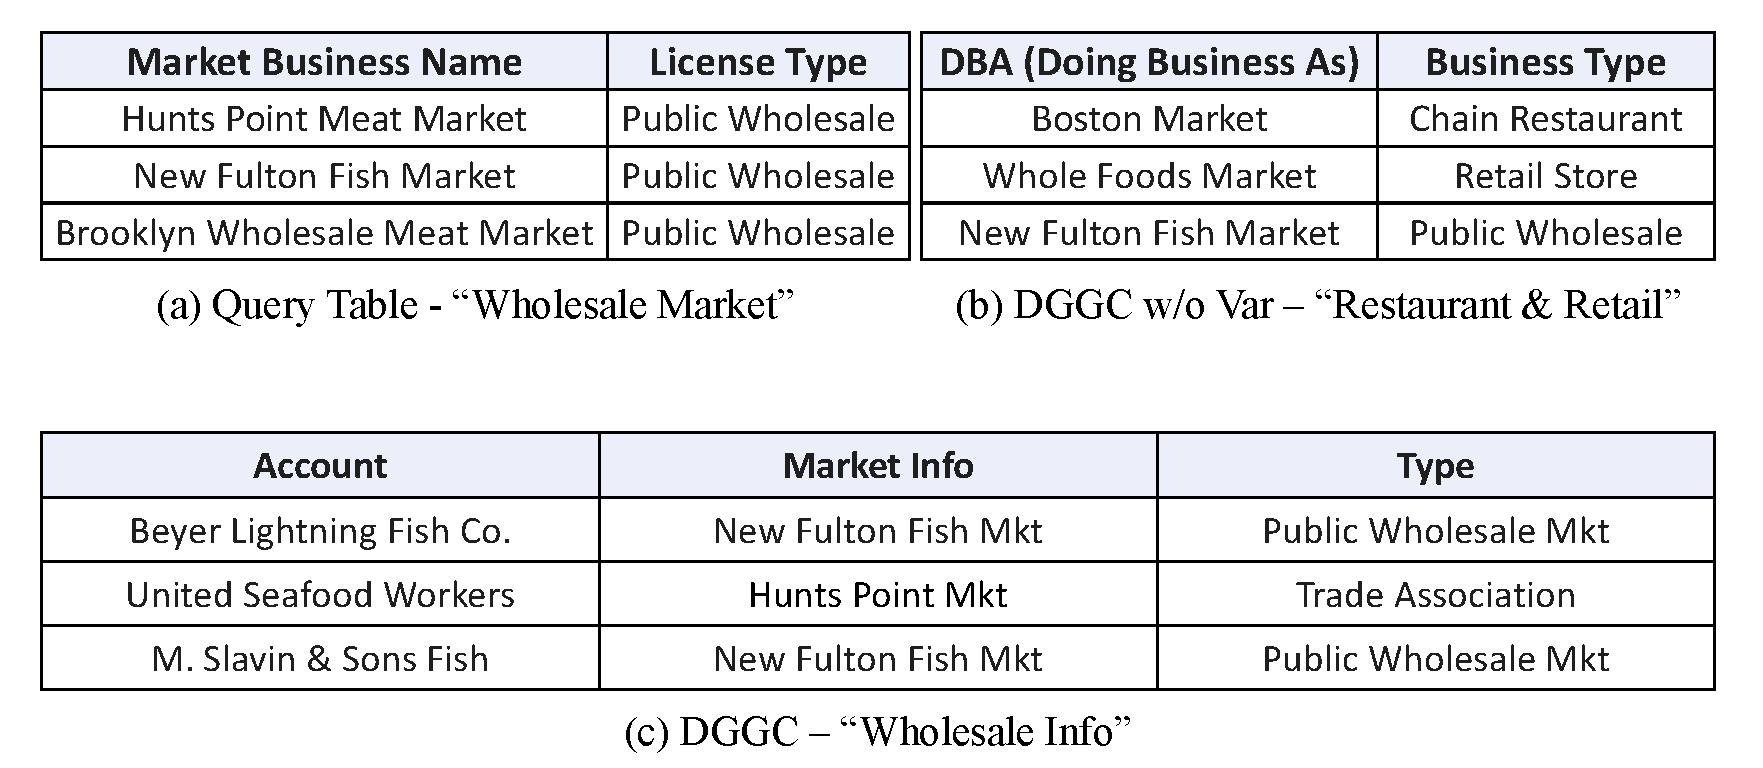
\includegraphics[width=1\linewidth]{figure/case_study.pdf}
    \caption{A case study of table union search: (a) The query table about ``Wholesale Markets''; (b) The returned table of DGGC w/o Var, which is a restaurant \& retail table due to its high lexical overlap with the query table (e.g., ``Market'', ``Type''); (c) The returned table of DGGC, which is a true positive containing markets with public whole sale type. }
    \label{fig:casestudy}
   
\end{figure}

To intuitively understand the superiority of our approach, we present a case study in Figure \ref{fig:casestudy} DGGC with the DGGC w/o Var. We analyze a representative query from the ``Wholesale Markets'' domain where lexical overlap introduces ambiguity.

As shown, the DGGC w/o Var model retrieves a ``Restaurant Inspection'' table as the top result. This occurs because the baseline relies heavily on keyword matching, thereby failing to capture the semantic boundary despite the severe lexical overlap (e.g., tokens like ``Market'' and ``Seafood''). Specifically, the point-based embedding projects these structurally different tables into close proximity due to shared high-frequency terms.



However, using the Wasserstein constraint (DGGC) successfully retrieves the correct target (\texttt{Wholesale Info.csv}). This suggests that our model effectively models the semantic variance of the schema. Specificall  y, the column \texttt{Account Name} in the query forms a distinct Gaussian distribution with low variance. While the baseline conflates this with the \texttt{DBA Name} in the restaurant table, the Wasserstein metric penalizes the alignment between these mismatched distributions. Thus, the transport cost \cite{peyre2019computational} required to align these distributions remains high, allowing the model to filter out the hard negative. This qualitatively confirms that modeling tables as probability distributions compensates for the limitations of simple semantic matching in high-ambiguity scenarios.



To intuitively understand the superiority of DGGC in handling semantic specificity in tables, we provide a case study focus on the tables about ``Wholesale Markets'', a domain where heavy lexical overlap frequently impacts the performance of union search. Figure \ref{fig:casestudy} presents the query table and the union search results by DGGC and DGGC w/o Var. Figure \ref{fig:case_study_epoch} shows the MAP of all queries, the cosine similarity between the mean embedding of the query table in the case study and its negative sample embedding as the epoch increases.

As illustrated in Figure \ref{fig:casestudy} and Figure \ref{fig:case_study_epoch}, the DGGC w/o Var retrieves a ``Restaurant \& Retail'' table, which is misled by severe value-level lexical overlap (estimated Jaccard similarity $\approx 0.42$). The overlapping strings, such as ``Hunts Point Meat Market'' vs ``Boston Market'', ``License Type'' vs ``Business Type'' create a high similarity between two tables. At Epoch 1, the cosine similarity between negative samples is notably high at 0.982. However, as training progresses, this similarity significantly drops to 0.2138 by Epoch 30. The overall MAP@k reaches its peak at Epoch 2 but subsequently begins to decline. This deterioration can be attributed to the model's neglect of semantic specificity due to the absence of a variance constraint. As a result, the model overfits to noise, leading to a gradual decrease in MAP@k performance, which falls from 0.9346 to 0.7054.

\begin{figure}[!htpb]
    \centering
    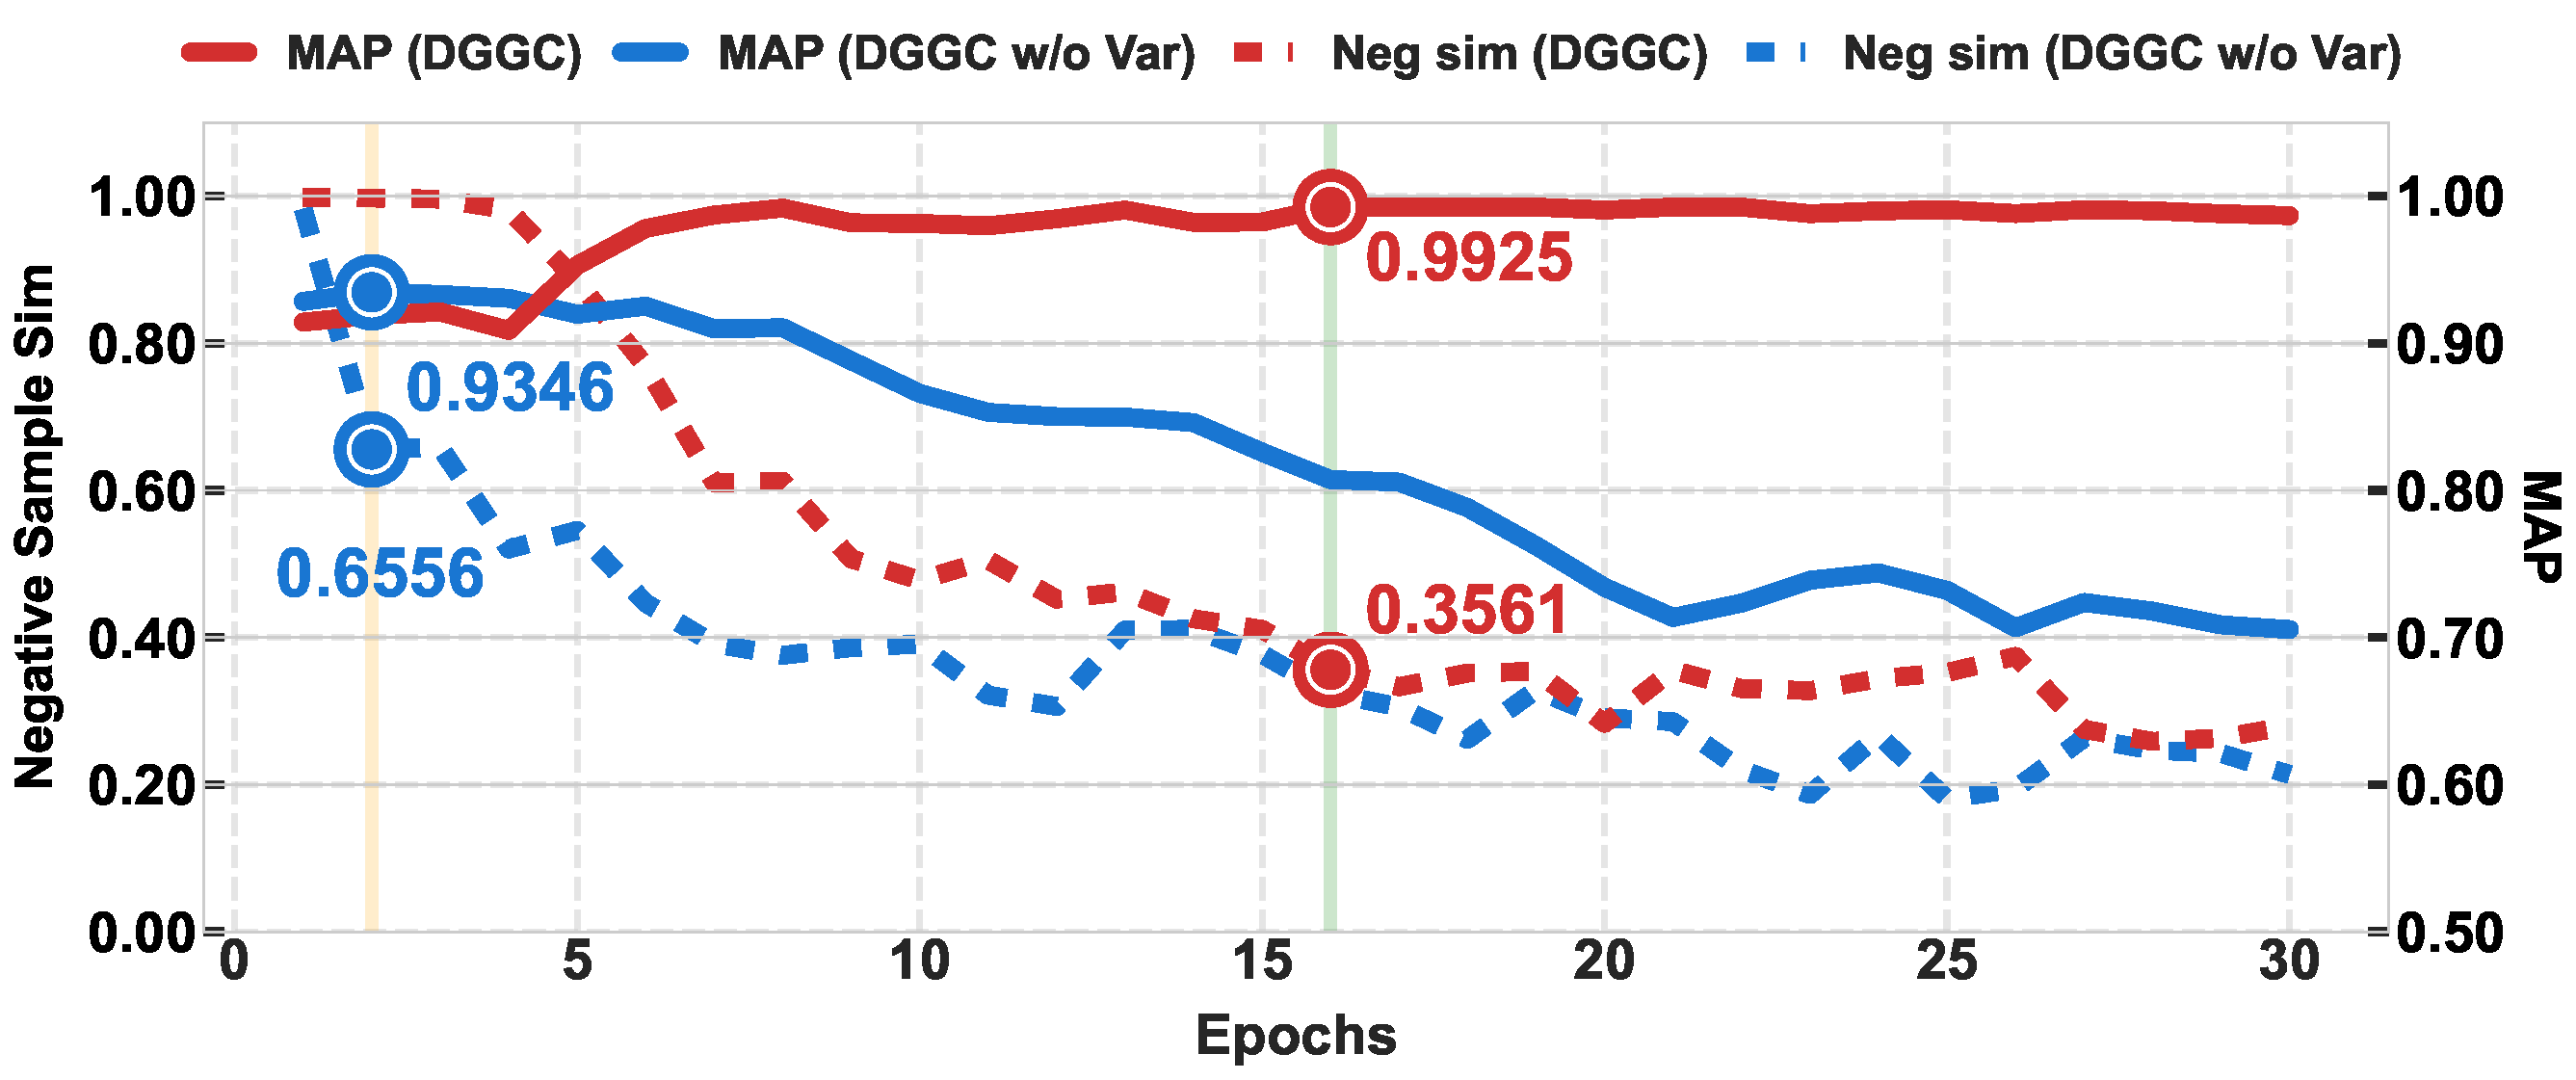
\includegraphics[width=.75\linewidth]{figure/case_study_epoch.pdf}
    \caption{The trend of cosine similarity among negative samples and the total MAP with the change of training epoch for the DGGC w/o Var and DGGC model. The light orange and light green vertical lines denote the epochs where the respective models achieve their optimal MAP performance. }
    \label{fig:case_study_epoch}
\end{figure}

In contrast, the DGGC model, which incorporates variance embeddings to account for semantic specificity, effectively captures the inconsistencies in table semantics illustrated in Figure \ref{fig:casestudy} (a) and (b). While both tables pertain to market entities, the query table emphasizes public wholesale markets, whereas Figure \ref{fig:casestudy} (b) focuses on more general contexts. The variance embedding in the loss function sensitively detects this mismatch. During training, the penalty term ($\lambda |\sigma_q - \sigma_n|_2$) in loss function actively separates the semantic centers, resulting in a significant reduction in cosine similarity from 0.9977 to 0.3561 (a 64.3\% decrease) between the tables while maintaining robust global performance, with MAP@k peaking at 0.9925. This successful filtering validates that introducing the variance constraint enables the model to distinguish between genuine semantic alignment \cite{karpukhin2020dense} and superficial lexical similarity \cite{robertson2009probabilistic}, which is critical for effective retrieval in real-world data lakes.

\fi



\end{document}
